\documentclass[a4paper, norsk, 11pt]{article}   
\usepackage[T1]{fontenc} 			                  % N�dvendig for fonter
\usepackage[latin1]{inputenc}                   % N�dvendig for ���
\usepackage[norsk]{babel}						            % Bruk norsk orddeling
\usepackage{graphicx}					                  % For � kunne inkludere grafikk
\usepackage{amsmath, amsfonts, amssymb}         % Pakker for � skrive matte
\usepackage[amssymb]{SIunits}                   % For � bruke \unit til SI-enheter
\usepackage{float}                              % For � bruke H som posisjon
\usepackage[bookmarks]{hyperref}                % For linker til kapitler
\usepackage{url}                                % For � bruke \url
\usepackage{array}                              % For � bruke m{1cm} p� tabell (midtstilt)

% Tegninger, som b�ndgap
\usepackage{tikz,tkz-tab}                       % Pakke til � tegne med i latex
\usetikzlibrary{decorations.pathmorphing}       % For � lage foton streker
\usetikzlibrary{decorations.pathreplacing}      % For � bruke kr�llparantes (brace)
\usetikzlibrary{shapes,arrows}                  % For � kunne tegne piler i tikz
\usepackage{xcolor}                             % Farger
\usepackage{rotating}                           % Rotere p� stash
\usepackage{subfigure}                          % Sette figurer ved siden av hverandre
\usepackage{epstopdf}                           % For at .eps figurer skal funke
\DeclareGraphicsExtensions{.pdf,.jpg,.png,.eps} % For � slippe � skrive extensions
\graphicspath{{./bilder/}}                      % For � slippe � skrive path til bilder

% Info om rapporten
\author{Jon Skarpeteig}
\title{Kryogen mikro-fotoluminiscense p� silisium solcellemateriale}
\date{\today}


%\setcounter{errorcontextlines}{\maxdimen} % Debug stuff

\begin{document}

% Tittleside
\begin{titlepage}
 \thispagestyle{empty}

% \maketitle
 
 \centering
 
 
\includegraphics[width=5cm]{NTNU-det-skapende_CMYK}
 
  \vspace{15mm} % Vertikalt mellomrom
 
    \Large
  {\bf{\textsl{TFE4530 - Fotonikk, Fordypningsprosjekt}}} \\
  
  % Tittel
  \vspace{25mm}          % Vertikalt mellomrom
  \huge
  \textbf{Kryogen mikro-fotoluminescense p� silisium solcellemateriale} \\
  \vspace{5mm}
  \textbf{av} \\
  \vspace{5mm}
 
  % Forfatter
  \large
  \textbf{Jon Skarpeteig} \\
  \vspace{25mm}

  \large
  \today \\
  \vspace{25mm}
  Veiledere: \\ Helge Weman \\ Arne R�yset \\
  \vspace{25mm} 
  \textsl{Norges Teknisk-Naturvitenskapelige Universitet} \\
  \textsl{Instittutt for Elektronikk og Telekommunikasjon} \\
  
\end{titlepage}

\pagenumbering{roman}

% Sammendrag
\begin{abstract}
%\section*{Sammendrag}

Tidligere fotoluminiscens m�linger gjort av Sintef p� multikrystallinsk silisium mangler s�kalte D-Linjer, som relaterer seg til dislokasjonslinjer og defekter for multikrystallinsk silisum. Disse defektene er kilder til tap for solceller. Det viser seg at det er flere kilder til tap i laboppsettet som ble tatt i bruk for b�lgelengder rundt 1550nm, eller 0,8eV. Det er disse b�lgelengdene som er mest interesante med tanke p� � kunne karakterisere tap i en pr�ve med silisium. Ved � utbedre laboppsettet fikk man mer enn tre ganger s� mye lys p� b�lgelengde 1530nm fram til spektrometeret.

Ved � se p� ulike posisjoner p� en pr�ve av multikrystallinsk silisium er det p�vist en posisjonsavhengighet p� spekteret. Ytterpunktene p� disse posisjonene er i et s�kalt bra omr�de, og et d�rlig omr�de. Et d�rlig omr�de har kilder til tap, som defekter, mens et bra omr�de hovedsaklig best�r av intrinsikk silisium.

Nye m�linger gjort p� en pr�ve med multikrystallinsk silisium ved lavtemperatur viser et spekter med dislokasjonslinjer, som ikke har v�rt observert ved hjelp av det gamle oppsettet. Det er ogs� kommet fram en topp som kan v�re relatert til forurensinger fra bor. Linjene som er omtalt som D3 og D4 kommer til syne. Linjene som omtales som D1 og D2, blir ikke observert. �rsaken til manglende D1 og D2 linjer er ikke kjent.
\end{abstract}

% Innholdsfortegnelser
\clearpage
\tableofcontents

%\addcontentsline{toc}{section}{Liste over figurer} % Legg til innholdsfortegnelse

\clearpage
\listoffigures

% Faktisk tekst til rapport
\clearpage
\pagenumbering{arabic}
\setcounter{page}{1}

\section{Introduksjon}

%%INCOMPLETE - mangler masse + stash er feil

Solceller er antatt � dominere energisektoren de neste hundre �r. For at dette skal bli tilfelle trengs det billige og effektive solceller. Multikrystallinsk silisium er materialet som har mest potensiale for � oppn� dette. Det er billig � produsere, men har ogs� relativt lav utnyttelse av solenergien. Derfor er det viktig � n�yaktig kunne identifisere kilder til tap, og forst� virkem�ten til slike materialer. 

Det er oppdrettet et laboratorium for � kunne gj�re m�linger p� slike celler ved hjelp av fotoluminisens p� ekstremt lave temperaturer. Tidligere m�linger av multikrystallinsk silisium p� dette laboratoriet viser deler av et spekter som er � finne p� tilsvarende m�linger (f.eks \cite{tarasov00}), men deler av tapsspekteret som var forventet dukket ikke opp. Dette prosjektet fokuserer p� hva som er �rsaken til dette avviket, og hvordan det kan utbedres. I tillegg til det er det fokusert p� virkem�te til solceller, og kilder til tap i multikrystallinsk silisium.
\clearpage
\section{Solcelle teori}

%TEORIDEL - Solceller - virkem�te, karakteristikker, MC vs. Thinfilm, utforming, 

De fleste solceller er krystallinske, det betyr at strukturen er ordnet, eller periodisk. I praksis vil krystallene inneholde feil av forskjellige slag. Noen solcellematerialer er ikke krystallinske, men mangler langtrekkende periodisitet. Disse best�r da av amorfe materialer.

Et fritt elektron i vakuum vil kunne innta en hvilken som helst energi. Et elektron i en krystallstruktur er bundet av energib�nd atskilt av gap med energitilstander som elektronene ikke kan ha. Det er derfor bare plass til et endelig antall elektroner i hvert b�nd, fordi hver tilstand bare kan romme to elektroner i f�lge Pauli-Prinsippet. For en krystall kan energib�ndene oppfattes som overlapp av enkelttilstander for hvert atom. En kan oppfatte energib�ndene som krystallens 'elektronskall'. 

\begin{figure}[!h]
 \centering
 	% Tegning
 	\begin{tikzpicture}[scale=0.5]
     	\draw[very thick,->] (1,6) -- node[below] {x}  (25,6); % X akse
    	\draw[very thick,->] (1,6) -- node[left] {\begin{sideways}Energi\end{sideways}} (1,18); % Y akse
    
    \begin{scope} % Valens og ledningsb�nd
		    \draw[thick,fill=black!10] (2,7) rectangle node {Valensb�nd} ++(22,4);
        \draw[thick,fill=black!10] (2,13) rectangle node {Ledningsb�nd} ++(22,4);
        \draw[thick,<->] (13,13) -- node[right] {B�ndgap} (13,11); % Pil
    \end{scope}
    \end{tikzpicture}    \caption{Energib�nd}
    \label{fig:energiband}
\end{figure}

Det �verste b�ndet kalles ledningsb�ndet. Energib�ndet umiddelbart under ledningsb�ndet, kalles valensb�ndet. De ikke tillatte tilstandene mellom valensb�ndet og ledningsb�ndet kalles b�ndgapet. Dette b�ndgapet er veldig viktig i forbindelse med solceller og oppgis ofte i elektronvolt (eV). % Legg til kr�llstash p� figur

For at elektronet skal kunne flytte p� seg m� det befinne seg i ledningsb�ndet. Et elektron m� ha nok energi til � kunne eksiteres fra valensb�ndet. Eksitasjon vil si at et elektron forflytter seg fra valensb�ndet til ledningsb�ndet. Dette kan skje ved at elektronet f�r h�y nok energi til � forflytte seg over b�ndgapet ved termisk energi, eller annen energi tilf�rt utenfra, som fra lys. Dette gir �kt ledningsevne til materialet. Samtidig blir det en ledig plass i valensb�ndet, som gj�r at andre elektroner i valsensb�ndet kan f� h�yere kinetisk energi p� grunn av f�rre kollisjoner. Dette p�virker ogs� materialet slik at det f�r h�yere ledningsevne.

Materialer deles ofte inn i tre kategorier; Isolatorer, halvledere, og metaller. Isolatorer har ingen, eller f� elektroner i ledningsb�ndet, som gir dem d�rlig ledningsevne. Metaller har som regel fylte ledningsb�nd ved romtemperatur, som gir dem god ledningsevne. Selv ved 0K har metaller et delvis fylt ledningsb�nd. Halvledere har d�rligere ledningsevne enn metaller, og vil ved 0K ikke ha noen elektroner i ledningsb�ndet. B�ndgapet til halvledere ligger mellom det for isolatorer og metaller, slik at ved romtemperatur er ledningsb�ndet delvis fylt, i motsetning til isolatorer.

\begin{figure}[!h]
 \centering
 % Tegning
 

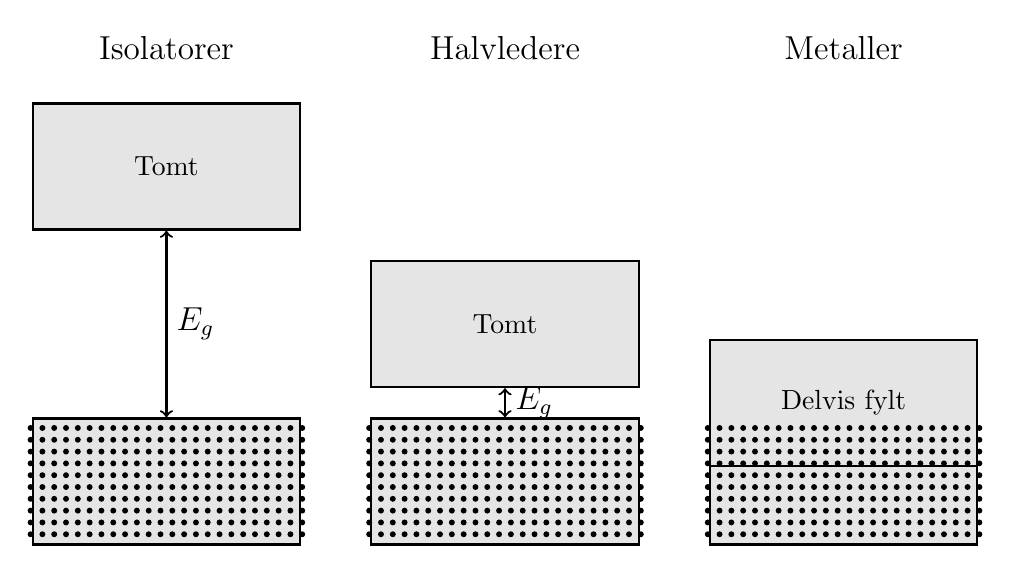
\begin{tikzpicture}
 	% Styles til elementer (kan ogs� v�re generelle utenfor tikzpicture)
	\tikzstyle{ledningsband} 	=	[rectangle, draw, thick, fill=black!10, text width=9em, text centered, minimum height=1.6cm]
	\tikzstyle{valensband}		= [rectangle, draw, thick, fill=black!10, text width=9em, text centered, minimum height=1.6cm]


	% Boksene i bunnen
	\node[valensband]	(valens_isolator)																										{};
	\node[valensband]	(valens_halvleder)	[right of=valens_isolator,  node distance=4.3cm]	{};
	\node[valensband]	(valens_metall)			[right of=valens_halvleder, node distance=4.3cm]	{};	
	
	% Boksene i toppen
	\node[ledningsband]	(lednings_isolator)		[above of=valens_isolator, 	node distance=4cm]	{Tomt};
	\node[ledningsband]	(lednings_halvleder)	[above of=valens_halvleder, node distance=2cm]	{Tomt};
	\node[ledningsband]	(lednings_metall)			[above of=valens_metall, 		node distance=1cm]	{Delvis fylt};
	
	% Piler
	\draw[thick,<->] (valens_isolator)  -- node[right] {\large $E_g$} (lednings_isolator);
	\draw[thick,<->] (valens_halvleder) -- node[right] {\large $E_g$} (lednings_halvleder);
	
	% Tekst p� toppen
	\node (isolator_tekst)  [above of=lednings_isolator,node distance=1.5cm]	{\large Isolatorer};
	\node (halvleder_tekst) [right of=isolator_tekst, 	node distance=4.3cm] 		{\large Halvledere};
	\node (metaller_tekst)  [right of=halvleder_tekst, 	node distance=4.3cm] 		{\large Metaller};
	
	% Elektroner i valensb�nd
	\foreach \y in {0,0.15,...,1.4}
		\foreach \x in {0,0.15,...,3.5} {
			\draw (\x-1.725,\y-0.67) circle (0.03cm) [fill=black];	% Isolator
			\draw (\x+2.575,\y-0.67) circle (0.03cm) [fill=black];	% Halvleder
			\draw (\x+6.875,\y-0.67) circle (0.03cm) [fill=black];	% Metall
		}	
	
\end{tikzpicture}

	    \caption{Typiske b�ndgap ved 0K} 
 \label{fig:bandgap}
\end{figure}
\vspace{30mm}

Typisk b�ndgap for halvleder silisium er 1.1eV, sammenlignet med 5eV for diamant som er en isolator. ~\cite[Kapittel 3]{streetman}

Hull er en beskrivelse for frav�r av elektroner i valensb�ndet. Et hull vil oppst� n�r et elektron eksiteres fra valensb�ndet til ledningsb�ndet. Lite b�ndgap, og h�y temperatur vil gi vesentlig flere elektroner i ledningsb�ndet, enn for lave temperaturer og stort b�ndgap. Dette beskrives med massevirkningsloven:

\begin{equation}
np=N_cN_ve^{-\frac{E_g}{kT}}
\label{eq:massevirkningsloven}
\end{equation}

der $n$ er antall elektroner, $p$ er antall hull, $N_c$ og $N_v$ er konstanter for gitte materialer. $E_g$ er b�ndgapet, $k$ er Boltzmanns konstant og $T$ er temperaturen i Kelvin. For en intrinsikk halvleder, det vil si en halvleder uten noe form for doping, for eksempel ren silisium, kan massevirkningsloven skrives:

\begin{equation}
np=n_i^2
\label{eq:massevirkningsloven_intrinsikk}
\end{equation}

der 

\begin{equation}
n_i=\sqrt{N_c N_v}e^{-\frac{E_g}{2kT}}
\label{eq:intrinsikk}
\end{equation}

Fra massevirkningsloven kommer det av $E_g$ er en avgj�rende faktor for om en krystall kan sies � v�re en halvleder eller ikke. 


\subsection{Doping}

Ved � sette inn andre atomer i en krystallstruktur, med en annerledes elektronfordeling er det mulig � �ke elektroner i ledningsb�ndet uten � endre konsentrasjonen av hull i valensb�ndet. Dette kalles donor-doping. Et eksempel p� donor-doping er � tilsette fosfor i en silisiumkrystall. Dette vil f�re til flere elektroner i ledningsb�ndet, da fosfor har et valenselektron mer enn silisium og valensb�ndet er tiln�rmet fullt. Fosfor vil i dette tilfellet kalles donor i denne donor-dopingen. Doping konsentrasjonen er vanligvis s� liten at b�ndstrukturen ikke forstyrres vesentlig. Hvis en for eksempel setter inn bor istedenfor fosfor, vil silisium krystallen bli akseptor-dopet. Bor har et mindre elektron i valensb�ndet enn silisium, og vil derfor tilf�re et hull ekstra i valensb�ndet. Som regel er donorkonsentrasjonen av hull og elektroner i henholdsvis valens- og ledningsb�nd vesentlig h�yere enn den intrinsikke, slik at det er en god tiln�rming � sette

\begin{equation}
n \approx N_d
\label{eq:donordoping}
\end{equation}

for donordoping, og

\begin{equation}
n \approx N_a
\label{eq:akseptordoping}
\end{equation}

for akspetordoping. Der $N_d$ er donorkonsentrasjonen, og $N_a$ er akseptorkonsentrasjonen.

En dopet halvleder omtales generelt som ekstrinsikk. Hvis en halvleder er dopet med overtall av donor atomer, har den overtall av elektroner, og kalles n-dopet. For akseptordoping omtales halvlederen som p-dopet, da den har overtall av hull. Den dominerende ladningsb�rertypen kalles for majoritetsb�reren. Majoritetsb�rerene vil v�re de som i hovedsak s�rger for str�mtransporten gjennom halvlederen.


\subsection{Transport- og rekombinasjons-prosesser}

Det er to mekanismer som bidrar til transport av elektroner og hull i halvledere: drift og diffusjon. Drift er transport av en ladd partikkel p� grunn av et elektrisk felt. For transport av et hull i en dimensjon er str�mmen $I_p$ lik antall hull $N_p$ ganger ladning $q$ som krysser et tverrsnitt.

\begin{equation}
I_p = N_p q
\label{eq:diffusjonsstrom}
\end{equation}

I vakuum vil et elektrisk felt akselerere hullene, og hastigheten vil stadig �ke. I halvledere vil det oppst� kollisjoner med atomene i halvlederen, som gir hullene en midlere hastighet s� lenge feltet er konstant. Denne midlere driftshastigheten er relatert til feltet via hullenes mobilitet $�_p$

\begin{equation}
v_p = �_p E
\label{eq:elektronfart}
\end{equation}

Hvis alle hullene beveger seg i samme retning kan en da beregne str�m per areal, eller str�mtetthet.

\begin{equation}
J_p = \frac{I_p}{A} = \frac{N_p q}{A} = pAv_p \frac{q}{A} = pv_p q = pq�_p E
\label{eq:hulltetthet}
\end{equation}

Kombinert med tilsvarende uttrykk for elektroner:

\begin{equation}
J = J_p + J_n = (nq�_n + pq�_p)E = \sigma E
\label{eq:stromtetthet}
\end{equation}

der $�_n$ er mobiliteten for elektroner, og $\sigma$ er halvlederens ledningsevne. $J_n$ er elektronstr�mtettheten.

Str�mmen blir da 

\begin{equation}
I = JA = A\sigma E = \left( \frac{A\sigma}{L}\right)V
\label{eq:strom}
\end{equation}

Halvledere vil typisk ha ledningsevne $10^{-8}$ til $10^3$ S\per\metre. Typiske verdien for isolatorer og metaller er henholdsvis $10^{-14}$ og $10^6$ S\per\metre ~\cite[Kapittel 4]{streetman}


%%%%%%%%%%% title?

Elektronet kan g� fra det ene b�ndet til det andre direkte eller indirekte. Ved indirekte generasjon og rekombinasjon kan elektronet benytte seg av s�kalte gap-tilstander. Dette er tilstander somer knyttet til forurensinger, defekter i krystallstrukturen, grenseflater mellom krystallkorn for multikrystallinske materialer, og overflater. Gap-tilstander ligger mellom valensb�ndet og ledningsb�ndet, som er ikke tillatte tilstander for en perfekt krystal (se fig. \ref{fig:indirekte})\\


\begin{figure}[!h]

\begin{tikzpicture}

% Styles til elementer
\tikzstyle{band} 	=	[rectangle, draw, thick, text width=12em, fill=black!10, text centered, minimum height=1em]
\tikzstyle{e} 	=	[circle, draw, fill=black] % radius=0.2cm
\tikzstyle{h} 	=	[circle, draw, fill=white] % radius=0.2cm

	% Direkte
	\node[band]	(direkte_valens)																									{};
	\node[band]	(direkte_lednings)	[above of=direkte_valens, node distance=3cm]	{};
	\node[e] (elektron1) [right of=direkte_valens] {}; % Elektron
	\node[h] (hull1) [left of=direkte_valens] {}; % Hull
	\node[e] (elektron2) [left of=direkte_lednings] {}; % Elektron
	\node[h] (hull2) [right of=direkte_lednings] {}; % Hull
	\draw[very thick,->] (-1,0.3) -- (-1,2.7) {} ; % Pil opp
	\draw[very thick,<-] (1,0.3) -- (1,2.7) {} ; % Pil ned
	\node (direkte_tekst) [rectangle, draw, text width=10em, below of=direkte_valens,node distance=1.5cm]	{\large Direkte generasjon og rekombinasjon};
	
	\node (lednings_tekst) [right of=direkte_lednings, node distance=3cm, text width=2em] {Ledningsb�nd};
	\node (valens_tekst) [right of=direkte_valens, node distance=3.2cm, text width=2em] {Valensb�nd};
	
	% Indirekte
	\node[band]	(indirekte_valens)		[right of=direkte_valens,  node distance=7.5cm]	{};
	\node[band]	(indirekte_lednings)	[above of=indirekte_valens, node distance=3cm]	{};
	
	\node[h] (h3) [left of=indirekte_valens, node distance=1.7cm] {}; % Hull
	\node[e] (e3) [above of=h3, node distance=1.5cm] {}; % Elektron
	\draw[very thick,->] (h3) -- (e3) {}; %Pil
	\draw[thick,-] (5.5,1.5) -- (6.1,1.5) {}; % Linje gjennom
	
	\node[e] (e4) [left of=indirekte_lednings, node distance=0.5cm] {}; % Elektron
	\node[h] (h4) [below of=e4, node distance=1.5cm] {}; % Hull	
	\draw[very thick,->] (h4) -- (e4) {}; % Pil
	\draw[thick,-] (6.7,1.5) -- (7.3,1.5) {}; % Linje gjennom
	
	\node[h] (h5) [right of=indirekte_lednings, node distance=0.5cm] {}; % Hull
	\node[e] (e5) [below of=h5, node distance=1.5cm] {}; % Elektron
	\draw[very thick,->] (h5) -- (e5) {}; % Pil
	\draw[thick,-] (7.7,1.5) -- (8.3,1.5) {}; % Linje gjennom
	
	\node[e] (e6) [right of=indirekte_valens, node distance=1.7cm] {}; % Elektron
	\node[h] (h6) [above of=e6, node distance=1.5cm] {}; % Hull	
	\draw[very thick,->] (h6) -- (e6) {}; %Pil
	\draw[thick,-] (8.9,1.5) -- (9.5,1.5) {}; % Linje gjennom
	
	\node (indirekte_tekst) [rectangle, draw, text width=10em, below of=indirekte_valens,node distance=1.5cm]	{\large Indirekte generasjon og rekombinasjon};
	
\end{tikzpicture}	

\caption{Generasjon og rekombinasjon}%
\label{fig:indirekte}%
\end{figure}


I halvledere med direkte b�ndgap, som GaAs, vil begge prosessene kunne opptre. Silisium har indirekte b�ndgap, og vil ikke f� en direkte prosess uten deltagelse av gittervibrasjoner (fononer). Dette er mindre sannsynlig enn indirekte generasjon og rekombinasjon, og indirekte generasjon og rekombinasjon vil derfor dominere. Elektronet antas � bevege seg som en planar b�lge med propageringskonstanten $\vec{k}$, ogs� kalt b�lgevektor.

% Figur fra side 69 streetman

Generasjons- og rekombinasjonsprosesser kan beskrives ved nettoproduksjon av elektroner til ledningsb�ndet, $U_n$, proposjonalt med avviket fra likevekt

\begin{equation}
U_n = - \frac{n-n^0}{\tau_n}
\label{eq:generasjon_n}
\end{equation}

der $\tau_n$ er midlere levetid for elektronet. $n$ er konsentrasjonene av elektroner, og $n^0$ er likevektskonsentrasjonene av elektroner. Midlere levetid, vil v�re den tiden elektroner er i ledningsb�ndet f�r det rekombinerer. Tilsvarende er nettoproduksjonen av hull $U_p$

\begin{equation}
U_p = - \frac{p-p^0}{\tau_p}
\label{eq:generasjon_p}
\end{equation}

der $p$ er konsentrasjonen av hull og $p^0$ er likevektskonsentrasjonen av hull. $\tau_p$ er midlere levetid for hull.


\subsection{Solceller}

En halvleder med et p-dopet og et n-dopet omr�de som ligger inntil hverandre kalles en pn-overgang. En slik pn-overgang har likerettende egenskaper. Det vil si at den leder str�m vesentlig bedre i den ene retningen enn den andre. Denne oppf�rselen definerer en diode. Siden p-siden har en konsentrasjon av elektroner i ledningsb�ndet som er vesentlig lavere enn n-sidens konsentrasjon av elektroner i ledningsb�ndet, oppst�r det transport av ledningsb�nd-elektroner fra n-siden til p-siden ved diffusjon. Det samme skjer ogs� for hull fra p-siden til n-siden. Denne str�mmen av ladnings kalles diffusjonsstr�mmen. I prinsippet kan ogs� dopantene Si, B og P diffundere mellom de to delene av krystallen, men er bare betydelig for veldig h�ye temperaturer, alts� ikke vesentlig i romtemperatur.

Deplesjonssjiktet er et omr�de n�r grenseflaten mellom de to dopekonsentrasjonene som vil v�re essensielt t�mt for frie ladningsb�rere. Siden n-siden av deplesjonssjiktet inneholder donorer uten tilh�rende elektron vil denne siden v�re positivt ladet, og tilsvarende vil p-siden v�re negativt ladet. Dette gj�r at det oppst�r et elektrisk felt fra n- til p-siden, eller et fall i potensial fra n-siden til p-siden. Dette feltet f�rer til en driftstr�m som g�r i motsatt retning av diffusjonsstr�mmen og f�rer til likevekt, alts� 0 netto str�m.

% figur fra s. 14 i kompendiet

\begin{figure}[H]%
\centering
\begin{tikzpicture}

	\tikzstyle{box} 	=	[rectangle, draw, thick, fill=black!10, minimum width=15em, minimum height=3cm]
	\tikzstyle{ladning} 	=	[circle, draw, fill=black!20, minimum size=0.6cm]
	\def\edistance{0.6cm}
	
	\node[box]	(p)	{p};
	\node[box]	(n) [right of=p, node distance=15em]	{n};
	
	\node[ladning] (p3) [right of=p, node distance=8.35em] 	{\tiny{+}};
	\node[ladning] (p2) [above of=p3, node distance=\edistance] {\tiny{+}};
	\node[ladning] (p1) [above of=p2, node distance=\edistance] {\tiny{+}};
	\node[ladning] (p4) [below of=p3, node distance=\edistance] {\tiny{+}};
	\node[ladning] (p5) [below of=p4, node distance=\edistance] {\tiny{+}};
	
	\node[ladning] (n3) [left of=n, node distance=8.35em] 			{\small{-}};
	\node[ladning] (n2) [above of=n3, node distance=\edistance] {\small{-}};
	\node[ladning] (n1) [above of=n2, node distance=\edistance] {\small{-}};
	\node[ladning] (n4) [below of=n3, node distance=\edistance] {\small{-}};
	\node[ladning] (n5) [below of=n4, node distance=\edistance] {\small{-}};
	
	% Draw curly braces using path decoration
	\draw [thick,decorate,decoration={brace,amplitude=5pt}]
   (2.2,1.6) -- (3.5,1.6)
   node [black,midway,above=2pt] {\footnotesize $|E|>>0$};

	\draw [thick,decorate,decoration={brace,amplitude=5pt}]
   (-2.8,1.6) -- (2.1,1.6)
   node [black,midway,above=2pt] {\footnotesize N�ytralt, $E=0$};

	\draw [thick,decorate,decoration={brace,amplitude=5pt}]
   (3.6,1.6) -- (8.5,1.6)
   node [black,midway,above=2pt] {\footnotesize N�ytralt, $E=0$};

	% Str�mpiler
	\draw [thick,<-] (2,-1.8) -- (3.6,-1.8) node [right=2pt]	{$I_{drift}$}; 
	\draw [thick,->] (2,-2.3) -- (3.6,-2.3) node [left=45pt]	{$I_{diffusjon}$}; 

\end{tikzpicture}

\caption{Deplesjonssjiktet}%
\label{fig:deplesjonssjiktet}%
\end{figure}

Ved belysning genereres det minoritetsb�rere i pn-overgangen utover dem som genereres termisk ved at fotoner eksiterer elektroner til ledningsb�ndet. Denne genereringen er ofte vesentlig st�rre enn driftstr�mmen. Denne str�mmen er uavhengig av potensialforskjellene i pn-overgangen. For en diode i m�rke er str�m-spenning karakteristikken:

\begin{equation}
I=|I_{drift}|e^{\frac{qV}{kT}-1}
\label{eq:diodeiv}
\end{equation}

N�r pn-overgangen blir belyst vil driftstr�mmen �ke, og forskyve str�m-spenning karakteristikken nedover

% figur fra side 22 i kompendiet
\begin{figure}[H]
\centering
\begin{tikzpicture}

	\draw [->] (-3,0) -- (3,0) node [right=5pt]	{V};  % Y-akse
	\draw [->] (0,-2) -- (0,3) node [above=5pt]	{I}; % X-akse

	% Diode
	\draw [dashed,-] (-3,-0.2) -- (-1,-0.2);
	\draw [dashed,-] (-1,-0.2) .. controls +(right:1.2cm) .. (1.5,3);
	\draw [->, >=triangle 45] (-2.5,0.5) -- node[right] {$I_{drift}$} (-2.5,0);
	\draw [->, >=triangle 45] (-2.5,-0.7) -- (-2.5,-0.2);
	
	% Solcelle
	\draw [-] (-3,-1.8) -- (-1,-1.8);
	\draw [-] (-1,-1.8) .. controls +(right:1.5cm) .. (1.5,2);
	\draw [<->, >=triangle 45] (-1.7,-1.8) -- node[right] {$I_{belysning}$} (-1.7,-0.2);

\end{tikzpicture}

\caption{Str�m-spenningskarakterisitikken for en solcelle}%
\label{fig:ivsolcelle}%
\end{figure}

For solceller defineres ofte str�m ut av cellen som positiv, slik at karakteristikken vendes om V-aksen

\begin{equation}
I=I_{belysning}-I_{drift}(e^{\frac{qV}{kT}-1})
\label{eq:solcelleiv}
\end{equation}

hvor $I_{belysning}$ er str�m generert av lys. Spenningen ved �pen krets er gitt ved:

\begin{equation}
V_{OC}=\frac{kT}{q}\ln(\frac{I_{belysning}}{I_{drift}}+1)
\label{eq:voc}
\end{equation}

Maks effekt som genereres av solcellen er gitt av:

\begin{equation}
P_m=I_m V_m
\label{eq:piv}
\end{equation}

Hvor $P_m$ er maks effekt, $I_m$ er maks str�m og $V_m$ er maks spenning. Fyllfaktoren FF er gitt av faktisk effekt ut, over teoretisk maks effekt:

\begin{equation}
FF=\frac{I_m V_m}{I_{belysning} V_{OC}}
\label{eq:fyllfaktor}
\end{equation}

hvor $V_{OC}$ er spenning ved �pen krets.

% fyllfaktor figur
\begin{figure}[H]
\centering
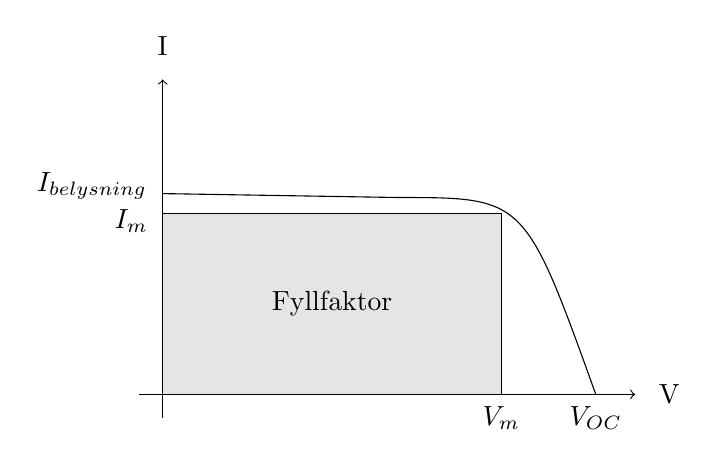
\begin{tikzpicture}

	\draw [->] (-0.3,0) -- (6,0) node [right=5pt]	{V};  % X-akse
	\draw [->] (0,-0.3) -- (0,4) node [above=5pt]	{I}; % Y-akse

	% Faktisk kurve
	\draw [-] (0,2.55) -- (3,2.5);
	\draw [-] (3,2.5) .. controls +(right:1.6cm) .. (5.5,0);
	
	% Fyllfaktor
	\node [draw, rectangle,fill=black!10,minimum height=2.3cm, minimum width=4.3cm] (FF) at (2.15,1.15) {Fyllfaktor};
	
	% Tekst
	\node at (-0.9,2.65) {$I_{belysning}$};
	\node at (-0.4,2.2) {$I_m$};
	\node at (4.3,-0.3) {$V_m$};
	\node at (5.5,-0.3) {$V_{OC}$};
	
	
\end{tikzpicture}

\caption{Str�m-spenningskarakterisitikk med fyllfaktor}%
\label{fig:fyllfaktor}%
\end{figure}

Virkningsgraden til en solcelle er representert ved $\eta$, som er gitt ved:

\begin{equation}
\eta=\frac{P_m}{P_{inn}}=FF \frac{I_{belysning} V_{OC}}{P_{inn}}
\label{eq:virkningsgrad}
\end{equation}

For multikrystallinsk silisium er den h�yeste virkningsgraden som er oppn�dd 18,9 \%. Dette ble oppn�dd av Mitsubishi 28. februar 2009 (fra pressemelding).
\subsection{Spektroskopi}

Spektroskopi benytter seg av fotoluminescens. N�r et elektronhullpar rekombinerer sendes energien som blir frigitt ut som et foton. Ved � m�le energien til fotonet kommer det fram hvor mye energi som ble frigitt under rekombinering. Dette sier noe om b�ndgapet til materialet, som igjen er en beskrivelse av hva slags materiale det er. Ved � belyse en pr�ve, med lys som har h�y nok energi og intensitet, vil det eksiteres lys til alle tilgjengelige tilstander. N�r disse tilstandene rekombinerer vil det sendes lys ut av pr�ven som kan fanges opp av et kamera og analyseres av en datamaskin for � f� ut et spekter av ulike b�lgelengder. For enkrystallinsk silisium er b�ndgapet 1.1eV, som f�rer til h�y intensitet av lys med 1.1eV energi.

\begin{figure}[H]
\centering
%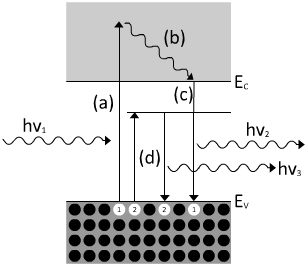
\includegraphics[width=10cm,bb=0 0 306 265]{luminisence.png}%
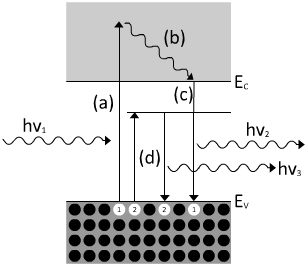
\includegraphics[width=10cm]{luminisence}%
\caption{Eksitasjon og rekombinering}%
\label{fig:luminisens}%
\end{figure}

Figur \ref{fig:luminisens} viser inkommende lys med h�y energi som eksiterer et elektron hullpar i $a$, som etter meget kort tid faller ned til en lavere energitilstand i $b$. I $c$ rekombinerer elektronet og det sendes ut et foton med energi lik $E_c$. Det andre elektronet som eksiteres i $d$ havner i en s�kalt "`trap"' state, hvor det kan befinne seg forurensninger eller defekter i en krystallstruktur. N�r dette elektronet rekombinerer sendes det ut et foton med lavere energi enn i $c$. Ved � se p� lyset som kommer ut fra en slik trap state kan det lokaliseres blant annet forurensninger. 

\subsubsection{Spektrometer}

For � kunne analysere ulike b�lgelengder m� man spre b�lgelengdene slik at de kan detekteres hver for seg. Dette kan gj�re ved hjelp av et spektrometer. Dette har en s�kalt diffraksjons-grating som f�rer til diffraksjon av lyset gitt ved:

\begin{equation}
d\sin(\theta _m)=m\lambda
\label{eq:grating_equation}
\end{equation}

Hvor $d$ er avstanden mellom spaltene i gratingen, $\theta _m$ er vinkelen til lyset, $m$ er et heltall for diffraksjonsordenen og $\lambda$ er b�lgelengden. I et spektrometer er det ofte mulig � bytte mellom flere ulike spalter. Spredningen er ofte begrensen, avhengig av hvor god oppl�sning man trenger. Dette f�rer til at en m�ling kun er innenfor et gitt intervall med en gitt senterb�lgelengde. For � f� ut et helt spekter, m� det gj�res flere m�linger med ulike senterfrekvenser.

\begin{figure}[H]
\centering
%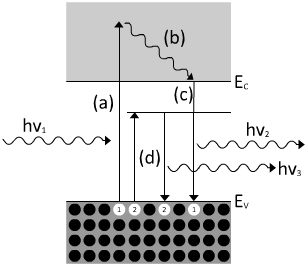
\includegraphics[width=10cm,bb=0 0 306 265]{luminisence.png}%
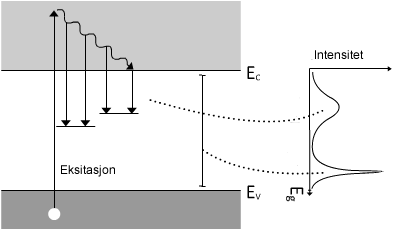
\includegraphics[width=10cm]{PL}%
\caption{Fotoluminisens}%
\label{fig:pl}%
\end{figure}

De ulike b�lgelengdene som kommer ut av pr�ven fanges opp av et kamera. Kameraet best�r av en endimensjonal rekke av detektorer, eller piksler, som fanger opp hver sin b�lgelengde avhengig av hvilke b�lgelengder som treffer hvilke piksler. Intensiteten og b�lgelengden til lyset registreres og lagres i en tabell som sendes til en datamaskin.

\subsection{Forventede verdier p� referansepr�ve}



\subsubsection{Forventet spekter for multikrystallinsk silisium}

Ved � se p� spekteret som fanges opp av kameraet er det mulig � relatere spekteret til fysiske egenskaper. Eksempelvis er spekteret for intrinsikk silisium kjent fra \cite{davies88}. For et s�kalt d�rlig omr�de er det if�lge \cite{tarasov00} fire tydelige spekter som kommer til syne p� multikrystallinsk silisium; D1, D2, D3 og D4 (se figur \ref{fig:dislokasjonslinjer})

\begin{figure}[H]
	\centering
			%\includegraphics[width=10cm,bb=0 0 512 297]{dislokasjonslinjer_tarasov00}
			\includegraphics[width=10cm]{dislokasjonslinjer_tarasov00}
		\caption{D-linjer}
	\label{fig:dislokasjonslinjer}
\end{figure}

Disse d�rlige omr�dene er antatt � v�re relatert til dislokasjonslinjer \cite{tarasov00} \cite{d-linje-temp} \cite{dislokasjoner85}. Hvilke energi disse linjene har, og hvor h�y intensitet som kommer ut er avhengig av tempetratur \cite{d-linje-temp}. Ved akustisk fonon-foton interaksjon i romtempratur blir det et bredere spekter som f�lge av ulike energier blant fononene som inng�r \cite{spekterbredning}. For � f� fram tydelige topper, gj�res m�linger ved temperaturer under -150$^\circ$C. Lave temperaturer er viktig for � kunne se individuelle topper, slik at de ikke forsvinner i termisk st�y som f�lge av fonon interaksjon med de dominerende karakteristikkene. 

\begin{figure}[H]%
\centering
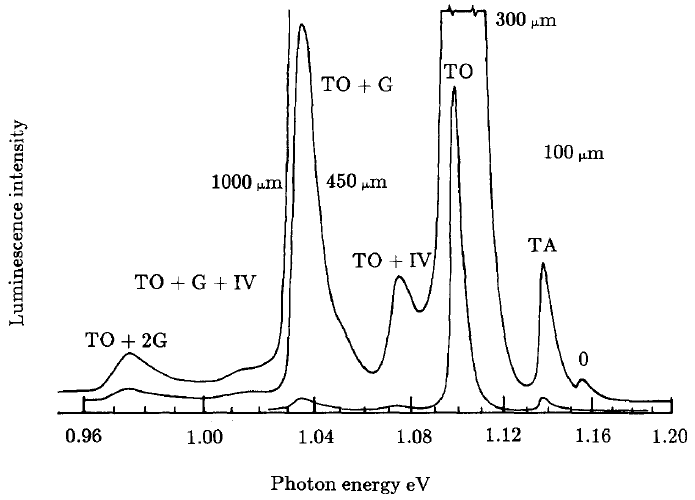
\includegraphics[width=10cm]{intrinsikk_silisium}%
\caption{Spekter for intrinsikk silisium fra \cite{davies88}}%
\label{fig:intrinsikk_si}%
\end{figure}

Disse m�lingene er gjort ved 28K med 4 ulike grating verdier mellom 100\micro m og 1000 \micro m. Labelene refererer til ulike fonon interaksjoner og modi.

\begin{table}[H]%
\centering
\begin{tabular}{|c|c|c|}
\hline
Energi & �rsak & Referanse \\
\hline
0.98eV & To fonon interaksjon (TA+2G) & \cite{davies88} \\
\hline
1.04eV & En-fonon interaksjon (TA+G) & \cite{davies88} \\
\hline
1.10eV & Transversal Optisk Mode (TO) & \cite{davies88} \\
\hline
1.14eV & Transversal Akustisk Mode (TA) & \cite{davies88} \\
\hline
1.16eV & Null-fonon komponent & \cite{davies88} \\
\hline
\end{tabular}
\caption{Forventede topper for et bra omr�de ved lavtempratur}
\label{tab:bra_omrade}
\end{table}

Transversal optisk mode ved ~1.125eV er b�ndgapet til silisium (ved 0K \cite{davies88}). Dette er hvor b�ndgapet til silisium ligger, og vil derfor dominere spekteret med tanke p� intensitet. 0.98eV og 1.04eV er kopier av den transversale optiske linja med henholdsvis to og ett fonon ekstra som assisterer rekombineringen. Transversal akustisk fonon-assisert rekombinering forventes ved 1.14eV. Ideelt sett skal det ikke v�re noe null-fonon komponent, men eksperimentelt kan dette observeres ved 1.16eV.

\begin{table}[H]%
\centering
\begin{tabular}{|c|c|c|}
\hline
0.8eV & D1 & \cite{mater08} \cite{sugimoto07} \cite{tarasov00} \\
\hline
0.9eV & D2 & \cite{mater08} \cite{sugimoto07} \cite{tarasov00} \\
\hline
0.95eV & D3 & \cite{mater08} \cite{sugimoto07} \cite{tarasov00} \\
\hline
1.00eV & D4 & \cite{mater08} \cite{sugimoto07} \cite{tarasov00} \\
\hline
1.04eV & En-fonon interaksjon (TO+G) & \cite{davies88} \\
\hline
1.1eV & B�nd til b�nd rekombinering (TO) & \cite{arguirov} \\
\hline
1.14eV & Transversal Akustisk Mode (TA) & \cite{davies88} \\
\hline
\end{tabular}
\caption{Forventede topper for et d�rlig omr�de ved lavtempratur}
\label{tab:bad_omrade}
\end{table}

D1-4 er dislokasjonsrelaterte linjer \cite{sugimoto07}. Disse er kun tilstede i et d�rlig omr�de. 1.1eV er fortsatt tilstede i et d�rlig omr�de, men med betydelig mindre intensitet enn et bra omr�de \cite{arguirov}. Det samme gjelder transversal optisk og akustisk fonon assisterte linjer ved 1.1eV og 1.14eV.
%\section{Tap}

Mye tap er relatert til s�kalte d�rlige omr�der, hvor det er mye rekombinasjon. Ved � karakterisere d�rlige omr�der, er det mulig � utbedre feil som det finnes kjente metoder for � unng�.

Fotoluminisensspekteret ved romtempratur er dominert av emisjon ved $h\nu_maks=1.09eV$, og et omr�de rundt $0.8eV$.  ~\cite{\tarasov00}

Et eksempel p� dette er fjerning av forurensinger som jern (?) CITATION NEEDED

\subsection{Dislokasjonslinjer}

Dislokasjonslinjer er linjer som kan ses p� spektrometri spekter av eksitert lys fra pr�ven

% dislokasjonsfigur

Det er fire linjer, D1, D2, D3 og D4 som hver har sin s�regne karakteristikk.

\begin{figure}[htbp]
	\centering
		\includegraphics{bilder/dislokasjonslinjer_tarasov00.PNG}
	\label{fig:dislokasjonslinjer}
\end{figure}


Figur \ref{fig:dislokasjonslinjer} viser dislokasjonslinjer for multikrystallinsk silisium ved 77K. D1' er ved 0.80eV, D2' ved 0.89eV, D3' ved 0.95eV og D4' ved 1.00eV \cite{tarasov00}

D1/D2 and D3/D4 belongs to different entities, based on the pl mapping.
\clearpage
\clearpage
\section{M�lemetode og Instrumentering}

En av utfordningene er � f� til et laboppsett som kan m�le og karakterisere ulike former for tap, slik som dislokasjonslinjer, forurensninger, og korngrenser. Dette er viktig for � kunne forst� �rsakene til tap, og for � kunne analysere hvilke framstillingsprosesser som gir et gunstig resultat.

\begin{figure}[H]%
\centering
	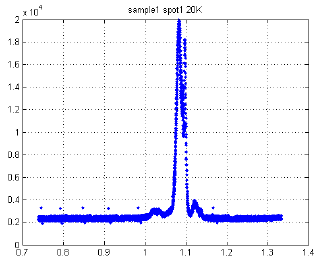
\includegraphics[width=10cm,bb=0 0 332 274]{bilder/cryolabtap.png}%
	\caption{Fotoluminisensspekter ved 20K i cryolab}%
	\label{fig:cryolabtap}%
\end{figure}

Publikasjoner som~\cite{tarasov00} (figur \ref{fig:dislokasjonslinjer}) viser et tapsspekter rundt 0,7-1 eV som ikke er synlig p� m�linger gjort p� cryolab. (figur \ref{fig:cryolabtap}) Grunnen til det er ikke kjent, men antas og v�re et resultat av tap i utstyr som linser og beamsplittere. 1eV tilsvarer 1240nm b�lgelengde fra ~\ref{eq:lysenergi}, som betyr at spekteret som antas � forsvinne har b�lgelengde 1100-1700nm.

\subsection{Laboppsett}
% laboppsett figur her

Eksitert lys fra pr�ven i figur \ref{fig:cryolabtap} g�r gjennom f�lgende komponenter:

\begin{table}[H]
\centering
\begin{tabular}{|c|c|c|c|}
\hline
1 & Vindu p� cryostaten & &  \\
\hline
2 & Objektiv & NT46-405 & \cite{Objektiv} \\
\hline
3 & Beam splitter & BS017 & \cite{beamsplitter} \\
\hline
4 & Linse & ACN127-020-B & \cite{old_lens} \\
\hline
5 & Linse & ACN127-020-B & \cite{old_lens} \\
\hline
6 & Linse & ACN127-020-B & \cite{old_lens} \\
\hline
7 & Spektrometer & iHR550 Imaging Spectrometer & \cite{spektrometer} \\
\hline
8 & Kamera & InGaAs Spectroscopy CCD & \cite{kamera} \\
\hline
\end{tabular}
\caption{Eksisterende lab oppsett p� cryolab}
\label{t:laboppsett1}
\end{table}


Det antas at det er flere kilder til tap blant komponentene som lyset skal gjennom f�r det n�r kameraet. Hoveddelen av tap kommer av refleksjoner, da de optiske komponentene ikke har vesentlig absorbsjon av lyset. Kameraet er oppgitt til � kunne h�ndtere 900 til 1700nm.

Den f�rste komponenten lyset skal gjennom er vinduet i kryostaten, det er oppgitt til � slippe gjennom over 90\% av lyset for b�lgelengder mellom 200nm og nesten helt opp til 2000nm. (Se figur \ref{fig:cryovindu} under vedlegg) Objektivet har en transmisjonfaktor p� rundt 60\% for b�lgelengder mellom 500 og 1800nm. Beamsplitteren er oppgitt til � dele str�len 50:50, med mindre enn 1\% refleksjon (tap) for b�lgelengdene 400-700nm. Men ut ifra figur \ref{fig:beamsplitter400-700nm} er det eksponensielt �kende for b�lgelengder over 700nm. I tillegg forsvinner 50\% av lyset i selve split prosessen. Linsene er oppgitt til � ha under 1\% refleksjon for b�lgelengder mellom 650nm og 1050nm, mens for b�lgelengder utenfor er det eksponensielt �kende refleksjon. Spektrometeret er oppgitt til � ha spektralt spekter fra 150 til 1500nm. 

Dette viser tydelig at beamsplitteren og linsene som er brukt i oppsettet er store kilder til tap, og b�r byttes ut for m�linger med b�lgelengder over 700nm.

\subsection{Forslag til nytt oppsett}

%Hvordan l�se problemet?

Det er tydelig at objektivet, beamsplitteren og linsene er kilder til store tap i systemet. For � kunne gj�re m�linger mellom 1\micro m og 1,5\micro m b�r disse byttes ut med komponenter som har begrenset med tap for de b�lgelengdene som er interessante. For � f� til et st�rre b�lgelengdeomr�de foresl�s det � sette opp en parallell veibane for b�lgelengder fra 1000nm og opp til 1500nm. Dette kan realiseres ved � sette opp speil i str�lebanen som manuelt kan flippes opp og ned for � kontrollere hvor lyset beveger seg.

Forslag til oppsett for parallell optisk vei:

% tegning av parallell veibane

Utstyr for � realisere dette oppsettet kommer fra \url{http://www.thorlabs.de}. F�lgende komponenter er valgt ut:

\begin{table}[H]%
\centering
\begin{tabular}{|c|c|c|}
\hline
Linse & LB4330 & \cite{new_lens} \\
\hline
Speil & PF10-03-P01-10 & \cite{speil} \\
\hline
Iris & ID12SS/M & \cite{iris} \\
\hline
Flip mount (for speil) & FM90/M & \cite{flipmount} \\
\hline
Beam Splitter & BS018 & \cite{beamsplitter_ny} \\
\hline
Post (bordskrue) & TR75/M & \cite{post} \\
\hline
Post holder & PH2/M & \cite{postholder} \\
\hline
Flip mount (for linse) & TRF90/M & \cite{flipmount_linse} \\
\hline
\end{tabular}
\caption{Utstyr til parallell lysbane}
\label{t:nytt_utstyr}
\end{table}

Linsa som er valgt ut skal i f�lge datablad klare over 90\% transmisjon helt opp til 2\micro m i motsetning til det forrige oppsettet. Da m�lingene som skal gj�res kan gj�res over et relativt stort omr�de p� pr�ven er det ikke s� farlig om det belyste omr�det ikke holder 100\% fokus, slik at et avvik p� noen grader i str�lebanen ikke er kritisk for resultatet. Det kun trengs en linse p� den parallelle banen for � fokusere inn til spektrometeret som alene gj�r at det blir mindre tap. Beamsplitteren er oppgitt til � ha mindre enn 0.3\% refleksjon for b�lgelengdene 1.1 til 1.6\micro m. Det vil fortsatt forvinne 50\% intensitet her p� grunn av at lyset splittes, men det frekvensavhengige tapet er i f�lge datablad mye mindre for disse b�lgelengdene. % legge til appendix / referere til figurer?

% laser b�lgelengde? for h�y intensitet til at tapet har s� mye � si?

Speil monteres p� en s�kalt 'flip mount', slik at det kan skrus fast i det optiske bordet i en bestemt posisjon, og vippes 90 grader inn eller ut av str�lebanen, slik at det blir en parallell optisk bane for lyset � f�lge n�r m�linger som antas � ligge over 1000nm skal gj�res.

%linser her ogs�?

% figur.

For � teste det nye lapoppsettet, er det tatt i bruk en pr�ve med Erbium som er gitt at skal lyse opp rundt 1550 (se fig. \ref{fig:erbium_eksitasjon}). Denne pr�ven har et absorbsjonsspekter som vist i figur \ref{fig:erbium_absorbsjon} som gj�r gr�nn laser p� 532nm s�rdeles godt egnet som pumpelys.

% Er absorbsjon figur

% Er eksitasjonfigur
\clearpage
\section{Resultater}

\subsection{Referansepr�ve i romtemperatur}

Figur \ref{fig:erbium_gammel} og \ref{fig:erbium_ny} viser Erbium referansepr�ve ved 300K, pumpet med 532nm laser, med grating lik 300.

%Erbium_gammel.eps
%Erbium_ny.eps

\begin{figure}[H]
\centering
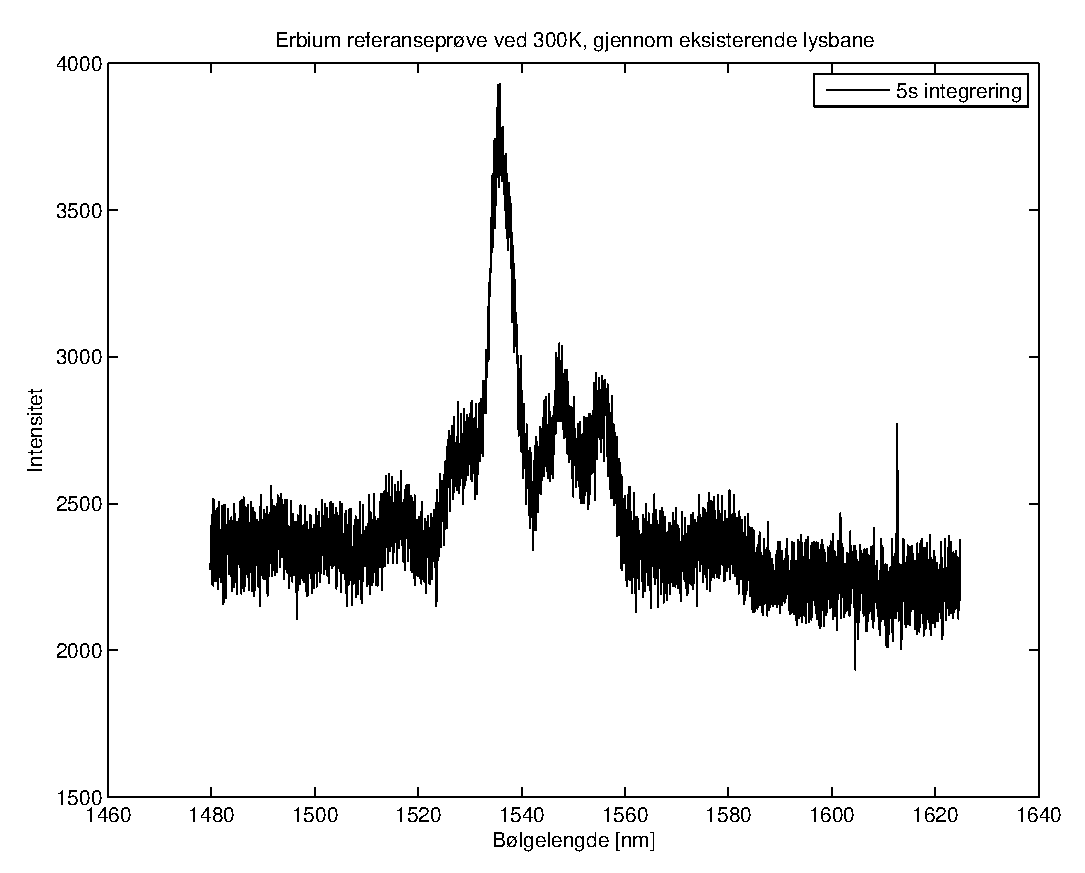
\includegraphics[scale=0.6]{Erbium_gammel.eps}
\caption[Eksitert lys sendt gjennom laboppsett brukt p� tidligere m�linger]{Eksitert lys sendt gjennom laboppsett brukt p� tidligere m�linger, med senterfrekvens rundt 1550nm}%
\label{fig:erbium_gammel}%
\end{figure}

\begin{figure}[H]
\centering
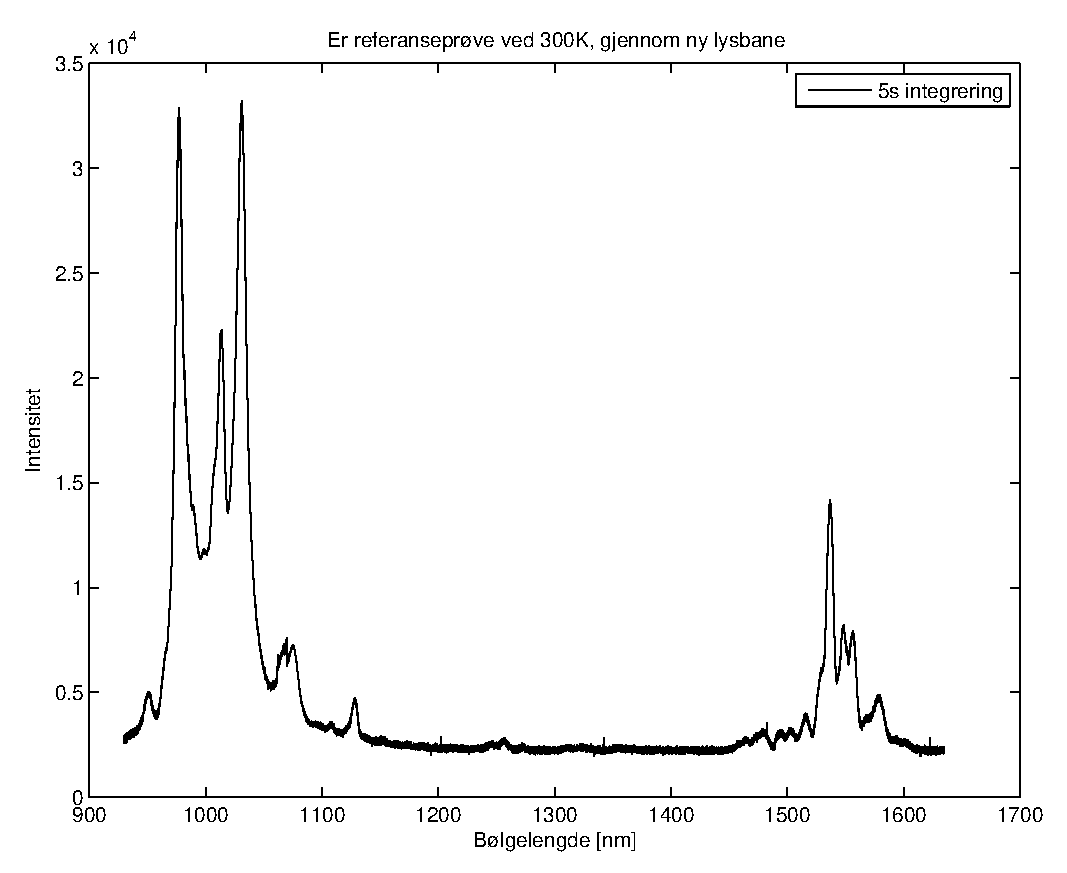
\includegraphics[scale=0.6]{Erbium_ny.eps}
\caption{Eksitert lys sendt gjennom nye komponenter}%
\label{fig:erbium_ny}%
\end{figure}

%Polert_300K.eps
%Upolert_300K.eps

\subsection{Polert og upolert pr�ve i romtemperatur}

Figur \ref{fig:upolert_sample} og \ref{fig:polert_sample} er m�linger gjort ved 300K, pumpelys lik 532nm, og grating lik 300. Den upolerte pr�ven er samme som i figur \ref{fig:cryolabtap}. Den andre pr�ven i figur \ref{fig:upolert_sample} er lik den upolerte i figur \ref{fig:upolert_sample}, bortsett fra at den er polert p� overflaten.

\begin{figure}[H]%
\centering
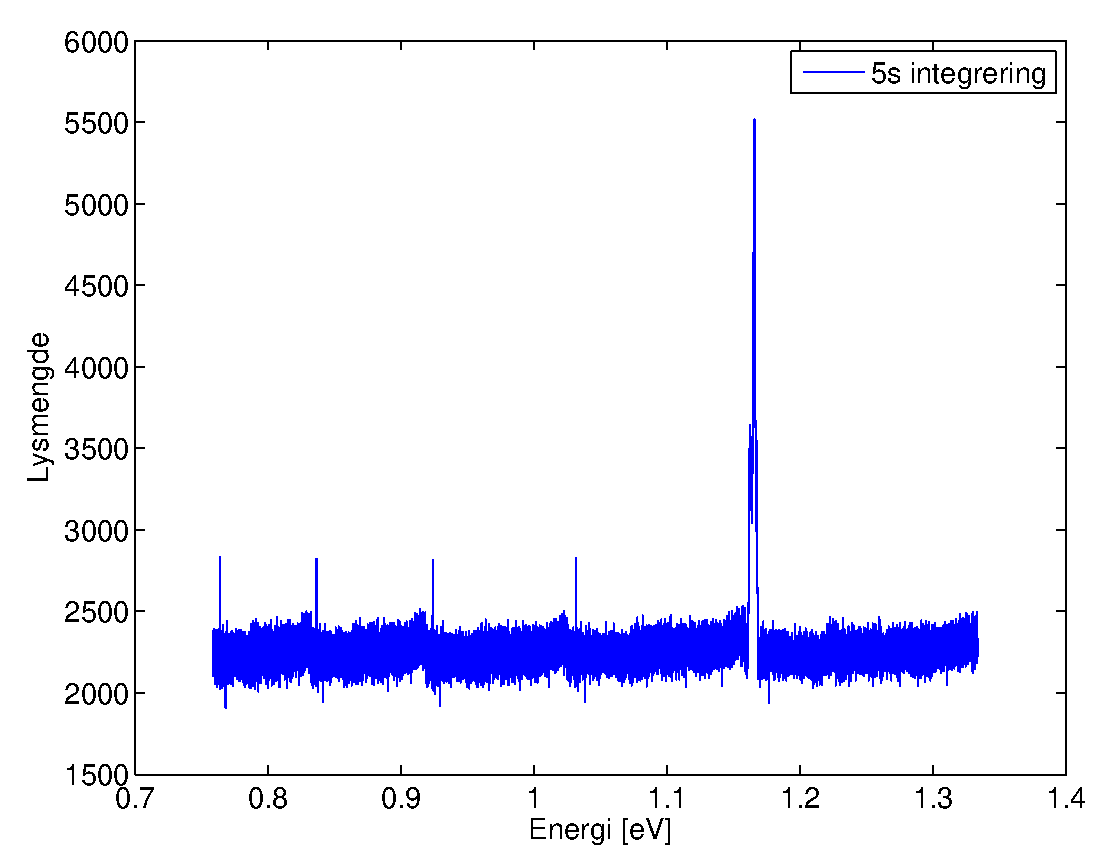
\includegraphics[scale=0.6]{Polert_300K.eps}
\caption{Polert multikrystallinsk silisium}%
\label{fig:polert_sample}%
\end{figure}

\begin{figure}[H]%
\centering
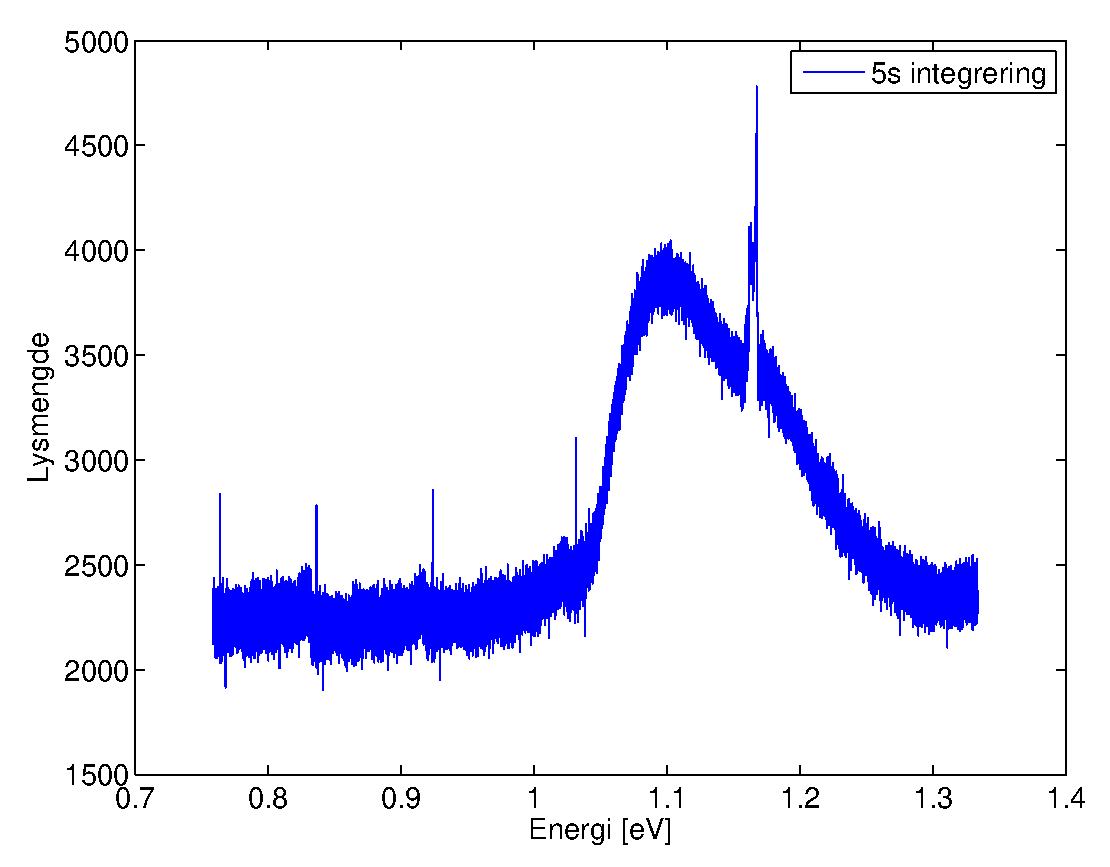
\includegraphics[scale=0.6]{Upolert_300K.eps}
\caption{Upolert multikrystallinsk silisium}%
\label{fig:upolert_sample}%
\end{figure}

\subsection{Sample 4 i romtemperatur}

\begin{figure}[H]%
\centering
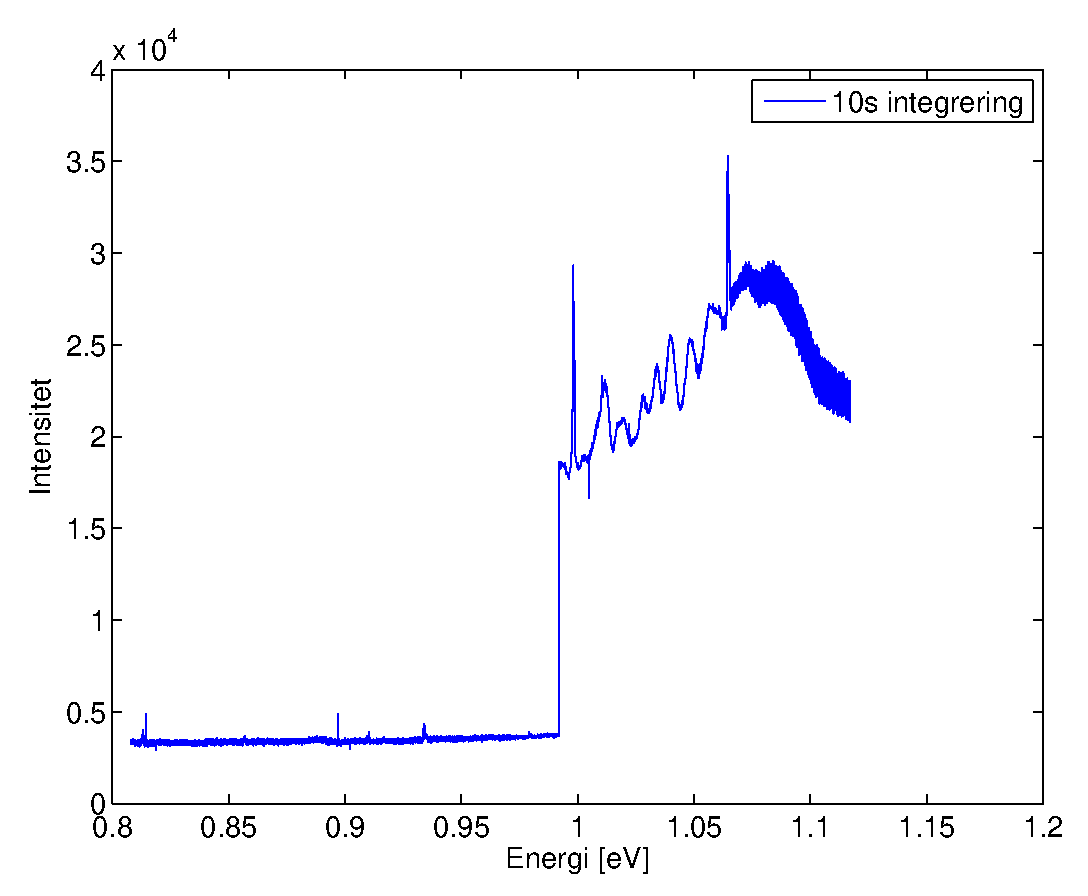
\includegraphics[scale=0.6]{Sample_4_romtemp_bad.eps}
\caption{Sample4 i et d�rlig omr�de}%
\label{fig:sample_4_romtemp_bad}%
\end{figure}

Figur \ref{fig:sample_4_romtemp_bad} bruker 60s integreringstid mellom 1 og 1,1eV

\begin{figure}[H]%
\centering
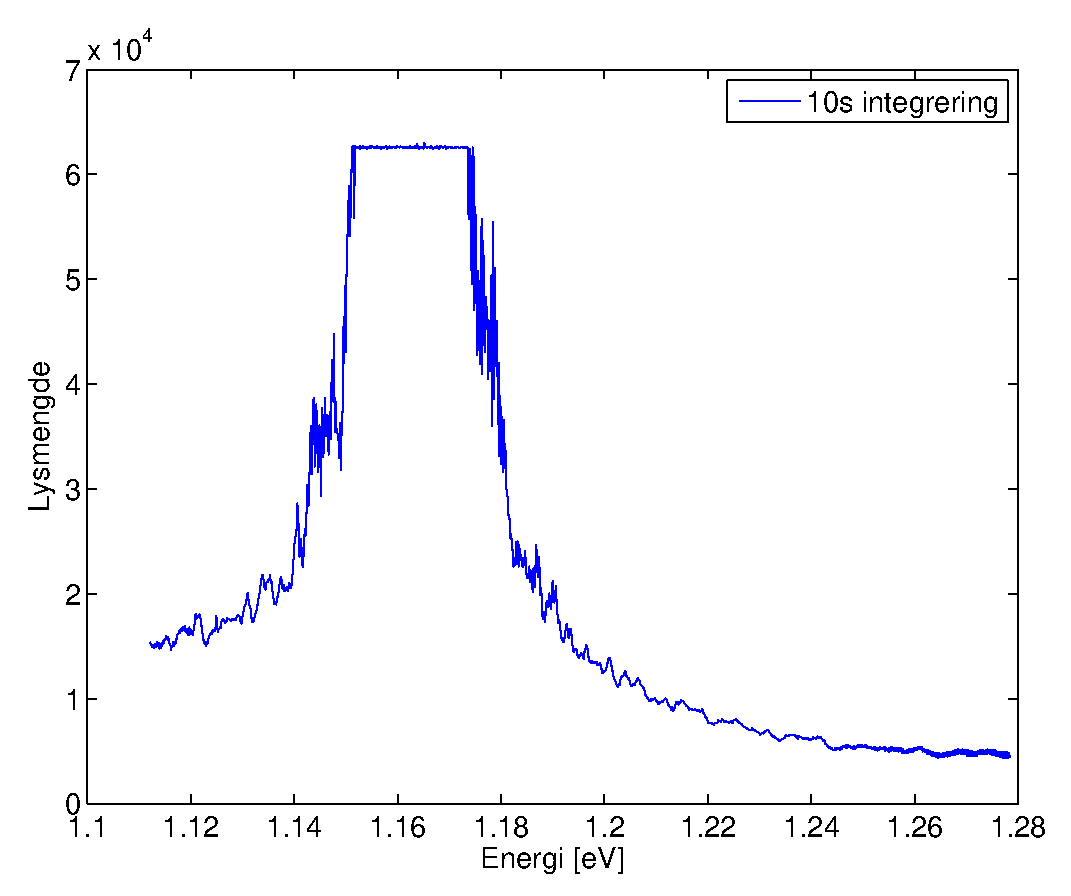
\includegraphics[scale=0.6]{Sample_4_romtemp_good.eps}
\caption{Sample4 i et bra omr�de}%
\label{fig:sample_4_romtemp_good}%
\end{figure}

\subsection{Sample 4 ved lavtemperatur}

Grating er satt til 300, og pumpelyset er fortsatt 532nm. Resultatene i figur \ref{fig:sample_4_2_1} og \ref{fig:sample_4_2_2} viser til samme punkt p� pr�ven.

\begin{figure}[H]%Sample_4.eps
\centering
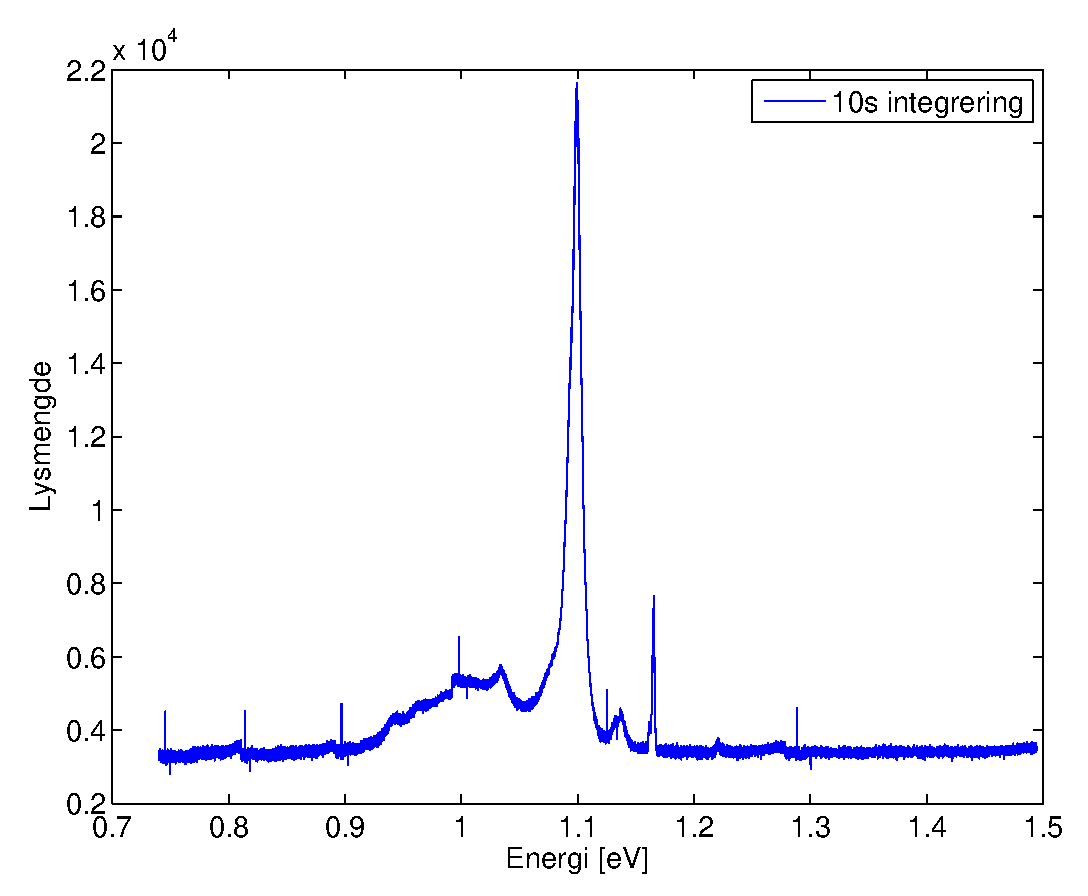
\includegraphics[scale=0.6]{Sample_4.eps}
\caption{Belyst med 13mW, ved 23K}%
\label{fig:sample_4_}%
\end{figure}

%Sample_4_1.eps
\begin{figure}[H]%
\centering
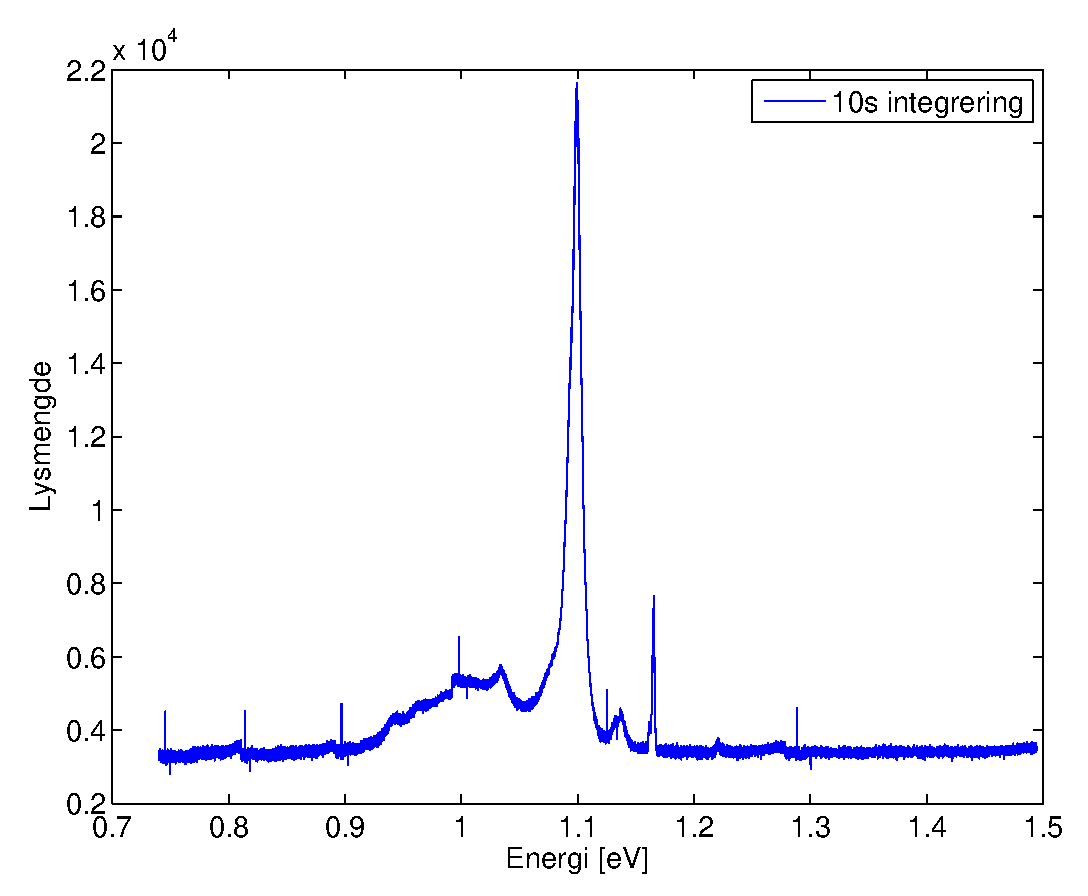
\includegraphics[scale=0.6]{Sample_4.eps}
\caption{Belyst med 4.6mW, ved 18K}%
\label{fig:sample_4_1}%
\end{figure}

%Sample_4_2_1.eps
\begin{figure}[H]%
\centering
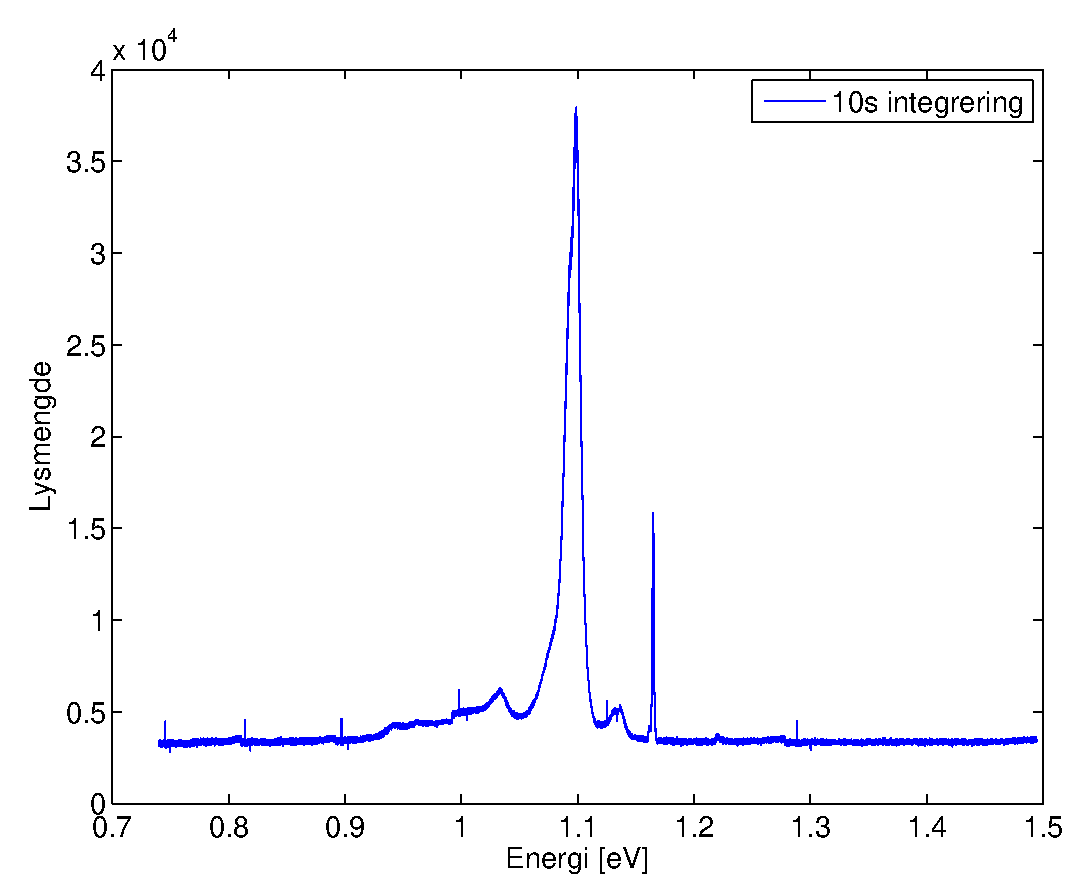
\includegraphics[scale=0.6]{Sample_4_2_1.eps}
\caption{Belyst med 15mW, ved 23K}%
\label{fig:sample_4_2_1}%
\end{figure}



\begin{figure}[H]%
\centering
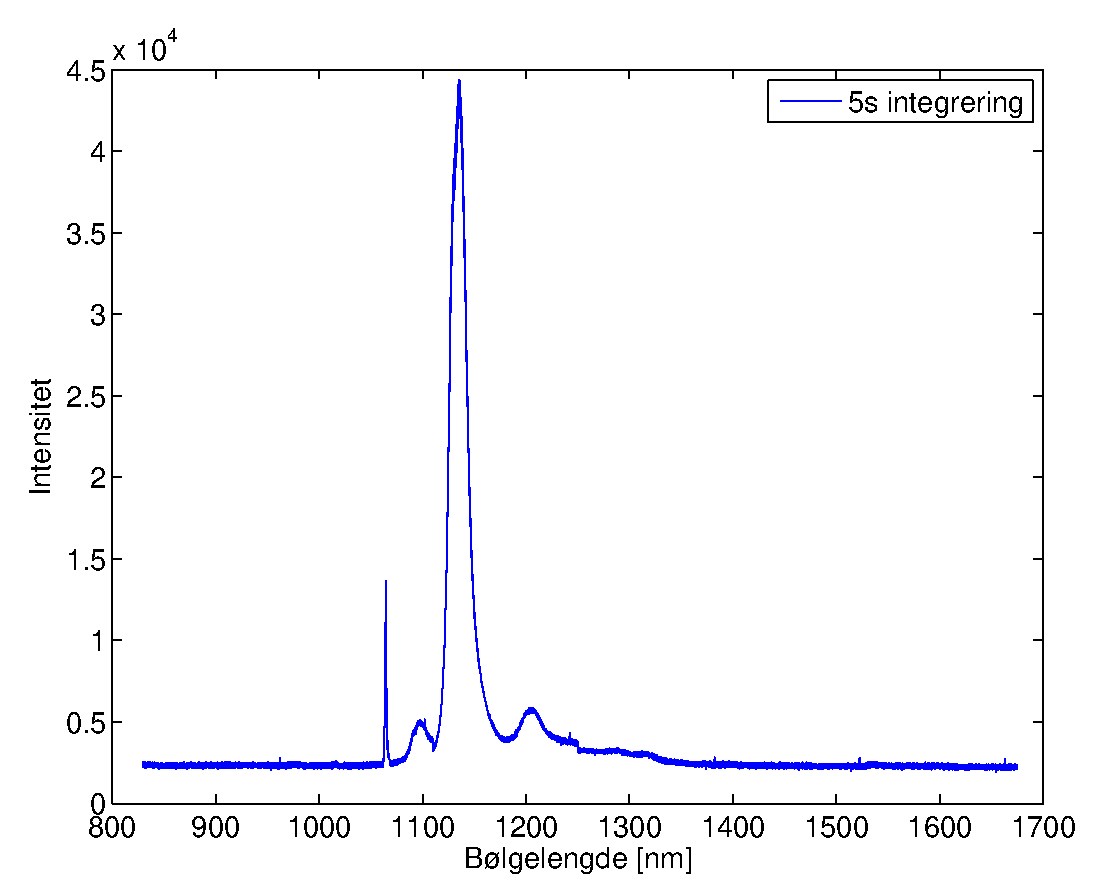
\includegraphics[scale=0.6]{Sample_4_2_2.eps}
\caption{Belyst med 30mW, ved 23K}%
\label{fig:sample_4_2_2}%
\end{figure}

%Posisjonsavhengighet.eps

\begin{figure}[H]%
\centering
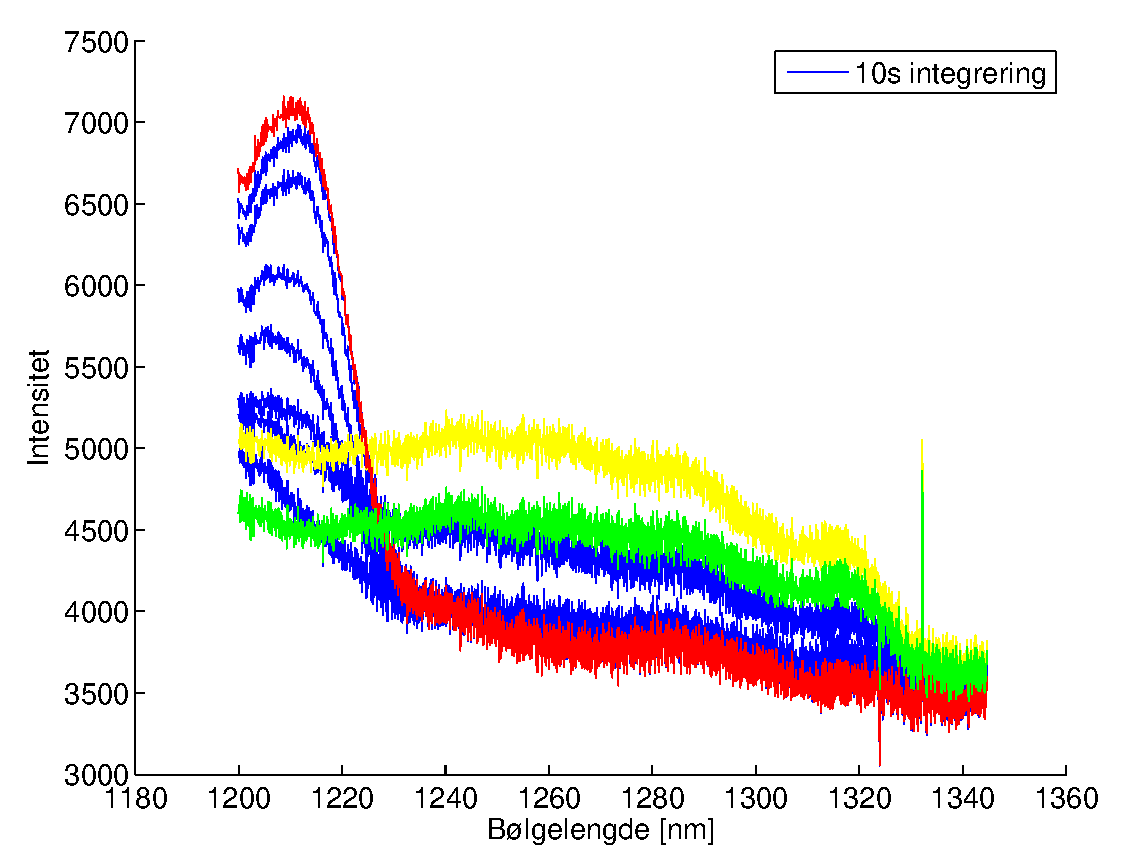
\includegraphics[scale=0.6]{Posisjonsavhengighet.eps}
\caption{Ulike posisjoner belyst med 13mW, ved 23K}%
\label{fig:posisjonsavhengighet}%
\end{figure}


% Sample4 bilde
\begin{figure}[H]%
\centering
%	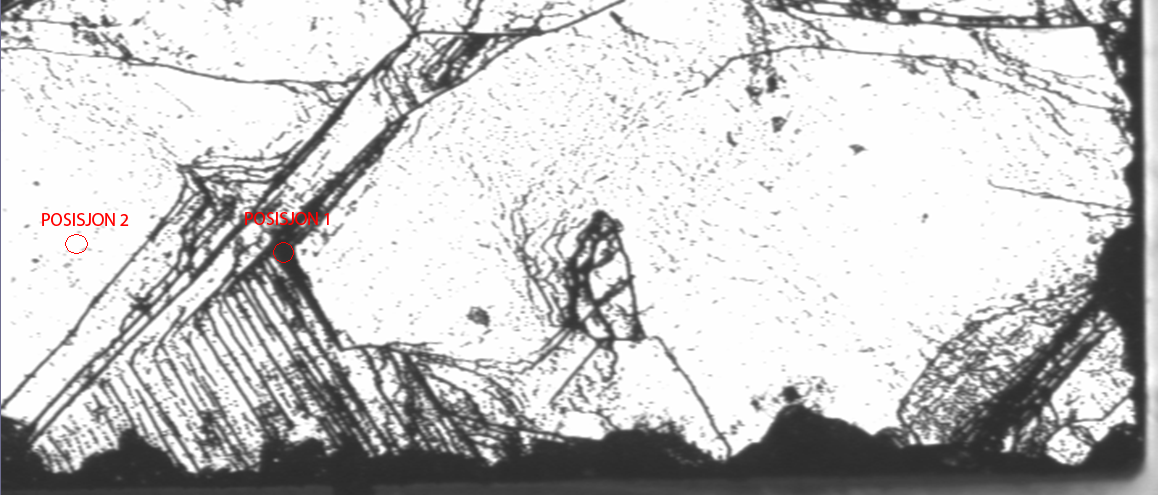
\includegraphics[width=15cm,bb=0 0 1158 495]{sample_4_edited.png}%
	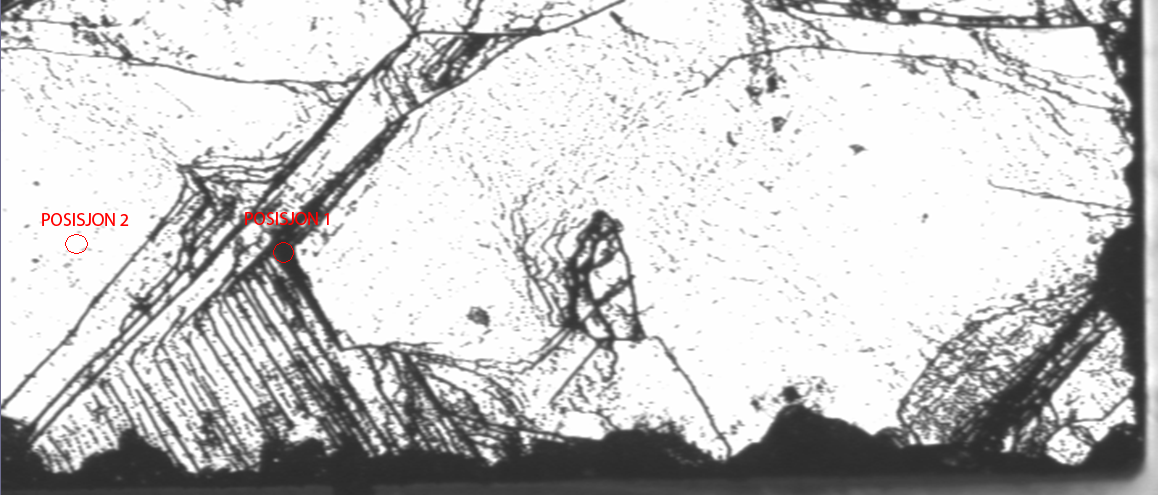
\includegraphics[width=15cm]{sample_4_edited.png}%
\caption{Posisjoner brukt for m�linger med lang integreringstid}%
\label{fig:sample4}%
\end{figure}


%Sample_4_SPOT_1_BAD.eps
\begin{figure}[H]%
\centering
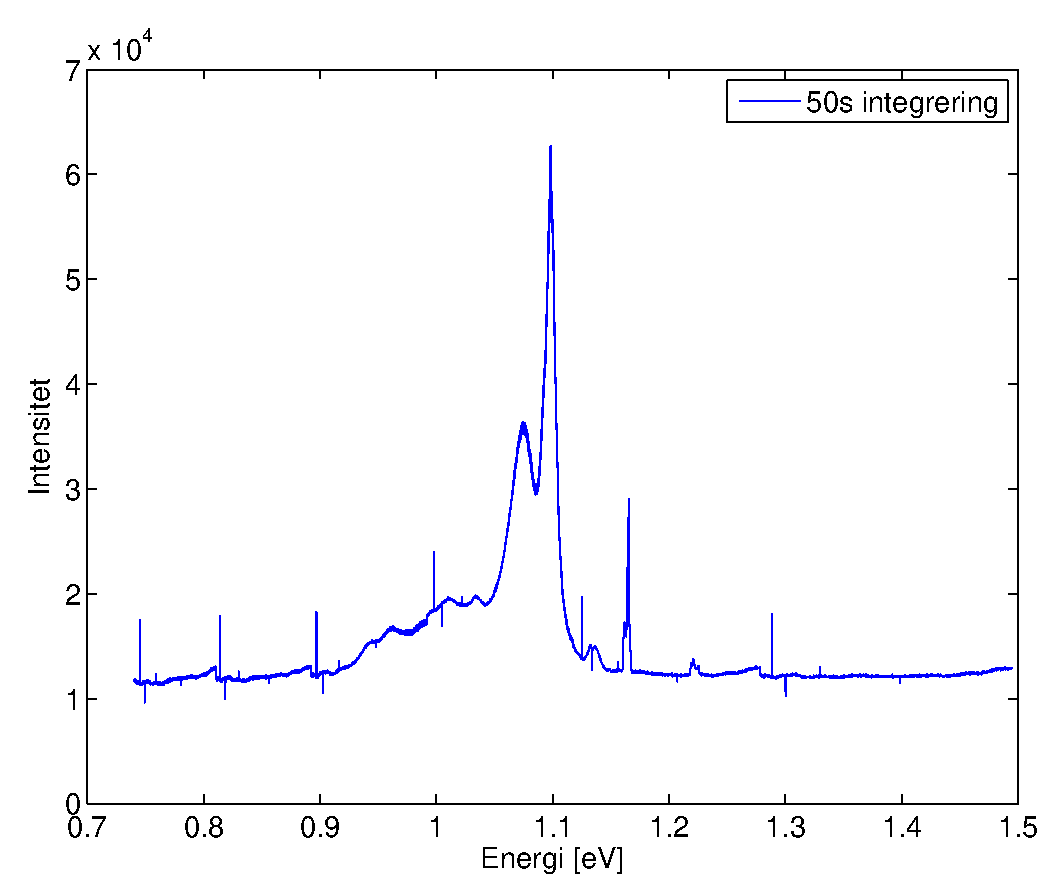
\includegraphics[scale=0.6]{Sample_4_SPOT_1_BAD.eps}
\caption{Resultatene fra posisjon 1 i figur \ref{fig:sample4}}%
\label{fig:bad_spot}%
\end{figure}

%Sample_4_SPOT_2_GOOD.eps
\begin{figure}[H]%
\centering
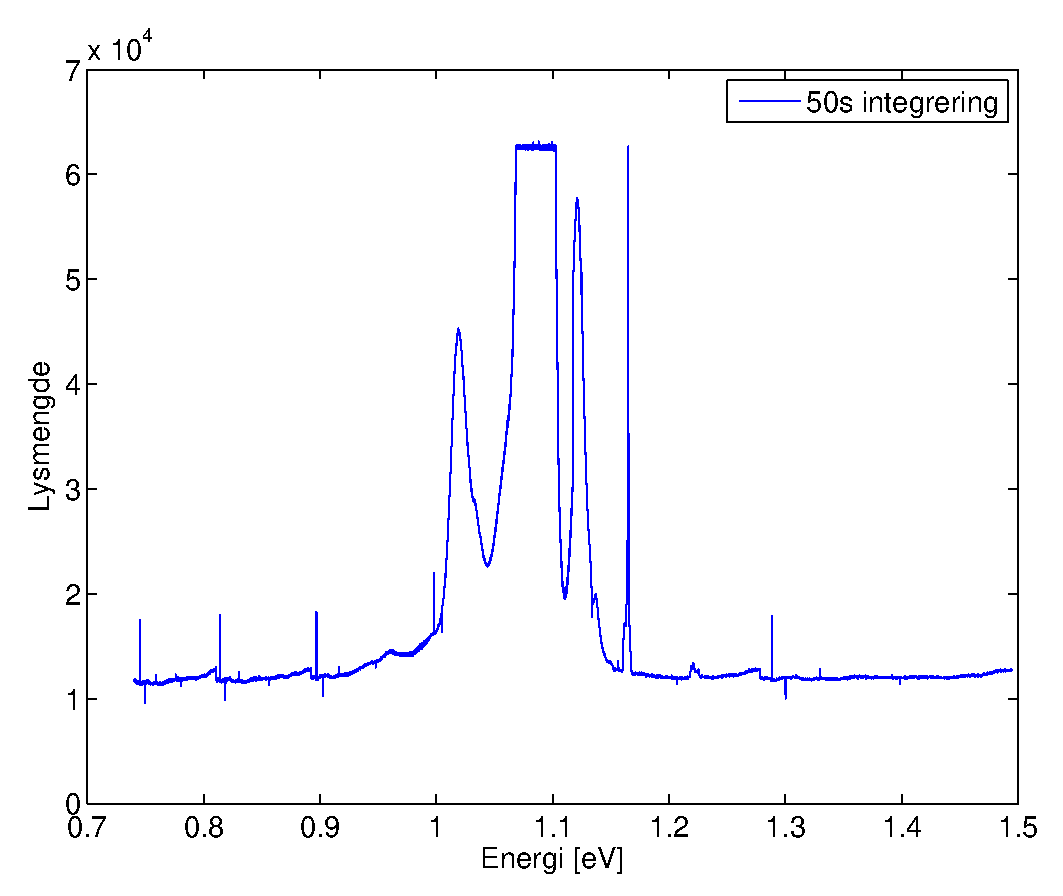
\includegraphics[scale=0.6]{Sample_4_SPOT_2_GOOD.eps}
%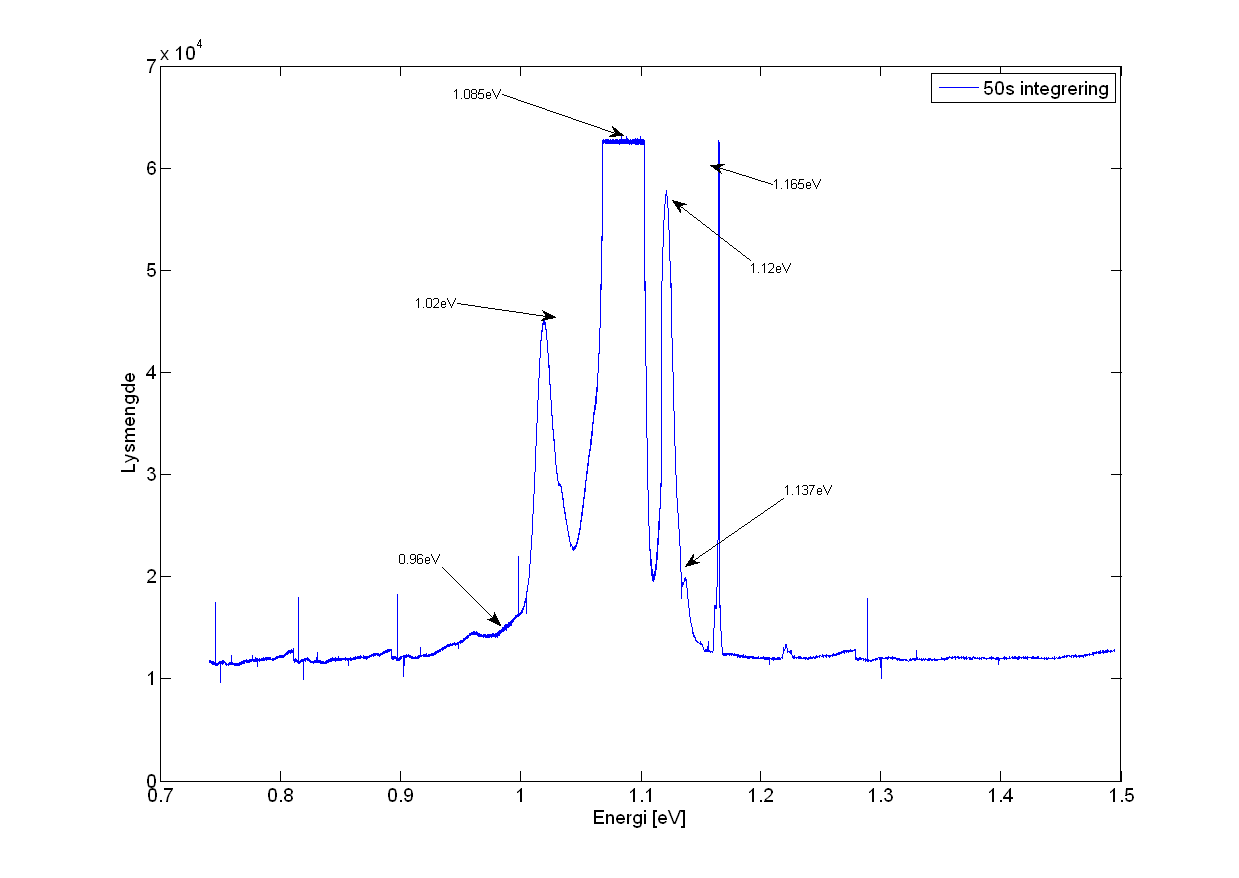
\includegraphics[width=12cm]{sample_4_cryo_good}
\caption{Resultatene fra posisjon 2 i figur \ref{fig:sample4}}%
\label{fig:good_spot}%
\end{figure}




\clearpage
\section{Diskusjon}

For � optimalisere laboppsettet ble det gjort m�linger hvert sekund, og utstyret justert slik at det ble h�yest mulig amplitude. H�yere amplitude viser til mindre tap i systemet. 

\subsubsection{Forbedring med nytt oppsett}

Emmitert lys fra referansepr�ven ble sendt gjennom gammelt oppsett, og nytt oppsett. De mest interessante b�lgelengdene befinner seg i omr�det rundt 1550nm, alts� ved 0,8eV. Det var p� forh�nd ventet en vesentlig forbedring for disse b�lgelengdene.

\begin{figure}[h]
  \hfill
  \begin{minipage}[t]{.45\textwidth}
    \begin{center}  
      	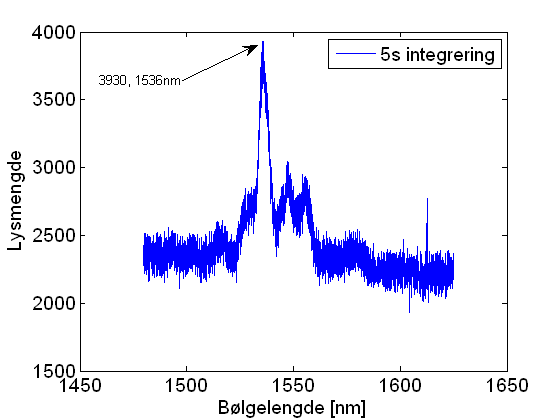
\includegraphics[width=\columnwidth]{referanse_gammel_piler.png}%
      \caption{Referansepr�ve gjennom gammelt oppsett}
      \label{fig:referanse_gammel_piler}
    \end{center}
  \end{minipage}
  \hfill
  \begin{minipage}[t]{.45\textwidth}
    \begin{center}  
      	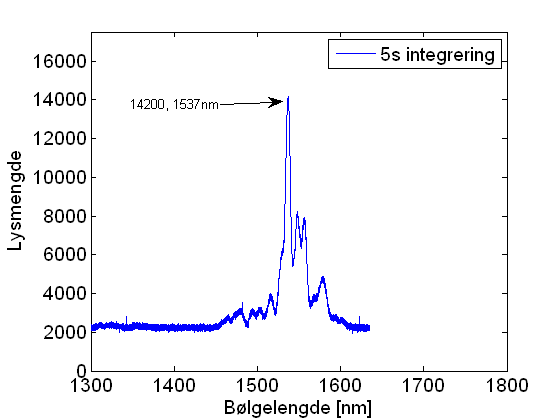
\includegraphics[width=\columnwidth]{referanse_ny_piler.png}%
      \caption{Referansepr�ve gjennom nytt oppsett}
      \label{fig:referanse_ny_piler}
    \end{center}
  \end{minipage}
  \hfill
\end{figure}


Figur \ref{fig:referanse_gammel_piler} og \ref{fig:referanse_ny_piler} viser at det nye utstyret gir mer enn tre ganger s� mye lys for b�lgelengder rundt 1550nm. Forventet resultat var fem ganger s� mye lys, men dette var basert p� en rekke antagelser om tap i eksisterende utstyr. Det nye oppsettet gir en klar forbedring for interessante b�lgelengder.

\subsubsection{Upolert og polert pr�ve i romtempratur}

Pr�ven i figur \ref{fig:polert_sample} er den samme polerte pr�ven som er gitt i figur \ref{fig:cryolabtap}. Det eneste som er tilstede her er andreordens diffraksjon fra laseren som kommer p� n�yaktig 1064nm. Hvorfor pr�ven ikke gir ut noe spekter er ukjent. Det antas � v�re feil i m�lingen som for eksempel feil fokus. Andre feilkilder kan v�re at pr�ven har en vinkel i forhold til sample holderen, eller at termisk pasta p� overflaten fra tidligere m�linger absorberer mesteparten av det eksiterte lyset. 

I figur \ref{fig:polert_sample} kommer det ogs� fram en tydelig karakteristikk ved 1064nm, som er det dobbelte av b�lgelengden til pumpelyset. Denne er altfor smal til � komme fra luminescensspekteret, og antas � komme fra andre ordens diffrasjon gitt av (\ref{eq:grating_equation})

Det er ogs� dukket opp enkeltst�ende "`spiker"' som ikke h�rer til noe kjent karakteristikk for silisium. Eksempelvis med senterfrekvens p� 1280nm viser en spiker verdiene:

\begin{table}[H]%
\centering
\begin{tabular}{|c|c|}
\hline
1341.950&2089.000 \\
\hline
1342.088&2419.000 \\
\hline
1342.225&2814.000 \\
\hline
1342.362&2338.000 \\
\hline
1342.499&2109.000 \\
\hline
\end{tabular}
\caption{Uregelmessig resultat ved 1342.2nm}
\label{t:uregel1}
\end{table}

Og med senterfrekvens p� 1420nm:

\begin{table}[H]%
\centering
\begin{tabular}{|c|c|}
\hline
1482.136&2089.000 \\
\hline
1482.272&2403.000 \\
\hline
1482.408&2822.000 \\
\hline
1482.544&2320.000 \\
\hline
1482.680&2140.000 \\
\hline
\end{tabular}
\caption{Uregelmessig resultat ved 1482.4nm}
\label{t:uregel2}
\end{table}

�rsaken til disse kan v�re et defekt piksel p� kameraet, da de dukker opp helt konsekvent p� samme sted i m�lingen rundt senterfrekvens + 62nm. Bredden p� disse er ogs� under 0.4nm, som er oppgitt n�yaktighet for spektrometeret \cite{spektrometer}.

Den upolerte pr�ven i figur \ref{fig:upolert_sample} er mer som forventet med bakgrunn i \cite{davies88}, med mesteparten av intensiteten rundt 1.1eV. Silisium har et indirekte b�ndgap, som gj�r at et elektron-hullpar ikke kan rekombinere uten hjelp fra et fonon. Ved romtemperatur har disse fononene h�yere termisk energi slik at et eksitert foton kan f� h�yere energi n�r det eksiteres via et slik fonon. Dette gir utslag p� spekteret ved at det blir en utbredning i energiniv�er p� detekterte fotoner. Refleksjoner fra laseren er ogs� vesentlig mindre her enn for den polerte pr�ven.

\subsection{Sample 4 i romtemperatur}
% hva skjer her egentlig??
M�lingene gjort i romtemperatur p� sample 4 er preget av mye st�y som en f�lge av h�y intensitet fra laseren. Sample 4 i figur \ref{fig:sample_4_romtemp_good} er gjort p� et s�kalt bra omr�de som hovedsaklig best�r av krystallinsk silisium. Her er det kun refleksjon fra laseren som er synlig. Det er samme resultat som for den polerte pr�ven i figur \ref{fig:polert_sample}. Det er fortsatt uklart hvorfor det ikke b�ndgapet til silisium kommer til syne her. Den polerte blanke overflaten reflekterer store mengder laserlys, som gir en kraftig spiker ved andreordens diffraksjonsm�nster. 

Intervallet fra 1eV til 1.1eV er tatt med lenger integreringstid, for � lokalisere toppen ved 1.1eV i et d�rlig omr�de. For et d�rlig omr�de (figur \ref{fig:sample_4_romtemp_bad}) er det antydning til en topp ved 1.1eV som tilsvarer b�ndgapet til silisium. D-linjene er ikke synlig i romtemperatur her i det hele tatt. Det er samme resultat som i \cite{sugimoto07}. Det ventes en topp tilsvarende den i figur \ref{fig:bad_spot}, bare bredere, men denne er sterkt p�virket av st�y. Ogs� her er refleksjoner fra laserlyset dominerende p� spekteret.

\subsection{Sample4 ved lavtemperatur}

Med bakgrunn i figur \ref{fig:posisjonsavhengighet} ble det gjort en m�ling i et s�kalt d�rlig omr�de, og en m�ling i et bra omr�de, med lang integreringstid. Et bra omr�de best�r hovedsakelig av intrinsikk silisium. Posisjonene er avmerket p� figur \ref{fig:sample4}. 

Ved m�linger p� 23K er det ikke lenger noe s�rlig utbredning i spekteret av fotoner direkte relatert til b�ndgapet til silisium. Det kommer til syne en karakteristikk med lavere energi som i f�lge \cite{tarasov00} er dominert av effekter i forbindelse med dislokasjonslinjer eller defekter i krystallstrukturen. Eksempelvis i figurene \ref{fig:sample_4_} og \ref{fig:sample_4_1}. I figur \ref{fig:posisjonsavhengighet} er det et utdrag av 20 m�linger gjort p� forskjellige lokasjoner p� Sample4. Her kommer det fram at denne karakteristikken er posisjonsavhengig. 

\begin{figure}[h]
  \hfill
  \begin{minipage}[t]{.45\textwidth}
    \begin{center}  
      	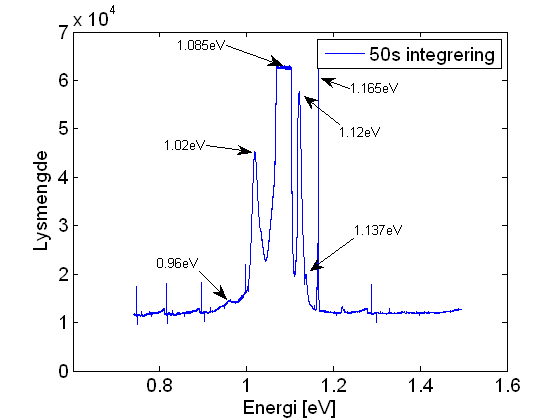
\includegraphics[width=\columnwidth]{sample_4_good_arrows.png}%
      \caption{Sample 4 for et bra omr�de}
      \label{fig:sample_4_good_arrows}
    \end{center}
  \end{minipage}
  \hfill
  \begin{minipage}[t]{.45\textwidth}
    \begin{center}  
      	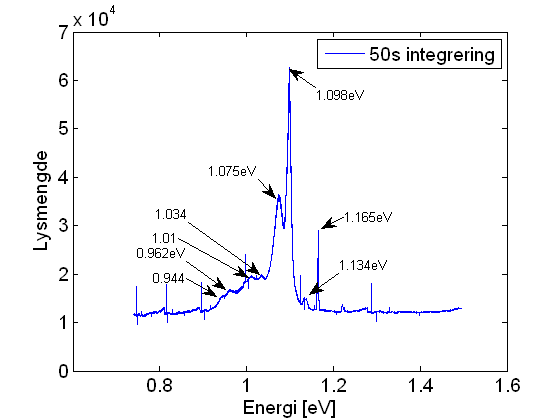
\includegraphics[width=\columnwidth]{sample_4_bad_arrows.png}%
      \caption{Sample 4 for et d�rlig omr�de}
      \label{fig:sample_4_bad_arrows}
    \end{center}
  \end{minipage}
  \hfill
\end{figure}

\subsubsection{Bra omr�de}

Sammenlignet med intrinsikk luminescense m�ling av silisium ved 26K gjort i \cite{davies88} stemmer figur \ref{fig:good_spot} veldig bra med forventende verdier. Hovedtyngden ligger rundt 1.1eV som blir kalt transversal optisk mode i \cite{davies88}. Dette er b�nd til b�nd rekombinering \cite{arguirov}. Med 50s integreringstid gikk kameraet i metning for denne b�lgelengden, men med bakgrunn i resultater fra figur \ref{fig:sample_4_2_1} og \ref{fig:sample_4_2_2} er det tydelig at denne karakteristikken er dominant ogs� her. Alts�, at mesteparten av energien ligger ved det indirekte b�ndgapet til silisium. Det er ogs� mulig at det er en TO + IV ved 1,075eV inne i denne toppen, det vil si p� venstre side av toppen, men b�nd til b�nd karakteristikken er for dominant til � kunne separere denne. Videre har fotonene assistert av to fonon (energi rundt 1.04eV) vesentlig h�yere intensitet enn for et d�rlig omr�de. Andre ordens diffraksjon fra laseren er som forventet. Omr�det som er karakteristisk for et d�rlig omr�de, som for eksempel ved dislokasjonslinjer, er ikke � finne i figur \ref{fig:good_spot}. I f�lge \cite{davies88} har det dukket opp en antydning til tre fonon assisterte fotoner rundt 0.96eV, transversal akustisk linje ved 1,12eV og en ideelt sett forbudt prosess der det ikke er noen fononer involvert med energier like over 1,14eV synlig som en liten topp. Toppene har et lite avvik p� rundt 0,1eV i forhold til \cite{davies88}. Det er mulig dette skyldes st�y, eller for lav oppl�sning. Resultatet er som forventet, uten store forskjeller.

\subsubsection{D�rlig omr�de}

Resultatene fra et d�rlig omr�de i figur \ref{fig:bad_spot} viser et bredt spekter rundt 1eV som ikke er synlig for et bra omr�de, som vist i figur \ref{fig:good_spot}. Resultatene fra \cite{tarasov00} viser til mye tydeligere topper for dette omr�det, som refererer til s�kalte D-linjer. Disse kommer ikke tydelig fram her. Mellom 0,9eV og 1,0eV er det antydning til topper som ofte omtales som D3 og D4 \cite{tarasov00} \cite{arguirov}. D3 er et fonon replika av D4 \cite{replica}. Linjene som omtales som D1 og D2 ser ut til � v�re helt borte. D3 og D4 er fra tabell \ref{tab:bad_omrade} ventet � v�re synlige ved henholdsvis 0,95eV og 1,00eV. Resultatet viser en topp ved 0,944eV og en ved 1,01eV. Toppen ved 1,01eV er ogs� h�yere enn toppen ved 0,944. Toppen ved 1,1eV er som ventet vesentlig lavere enn for et bra omr�de. Det samme er fonon replikert topp ved 1,034eV (ventet ved 1,04eV). Det er ogs� antydning til en tre-fonon assisert topp ved 0,962eV, som ligger p� akkurat samme energi som for et bra omr�de. Det samme gjelder toppen ved 1,134eV som for et bra omr�de relaterer seg til null-fonon interaksjon. Det er en topp ved 1,075eV som for intrinsikk silisium er TO + IV. Denne var ikke ventet � se med s� h�y intensitet. Det er mulig at den er like sterkt tilstede ved b�nd til b�nd karakteristikken ved 1,1eV for intrinsikk silisum, og at denne karakteristikken f�rst blir synlig n�r 1,1eV toppen blir liten nok. Det er et lite avvik i forhold til forventede resultater ogs� her. En forklaring kan v�re at posisjon og temperatur til d-linjene er avhengig av temperatur \cite{d-linje-temp}. 

D1 og D2 linjene er ikke � finne p� spekteret i det hele tatt. Disse er antatt � ha noe med hverandre � gj�re \cite{tarasov00}. \cite{arguirov} antyder at D1 og D2 linjene kan ha noe � gj�re med lokale fenomen, som materialstress. Hva som gir disse linjene er ikke kjent, men antas � v�re relatert til dislokasjoner. \cite{sugimoto07} viser at D1 linja ofte dominerer spekteret her, med relativt bred utstrekning. Dersom linjene hadde v�rt tilstede, er det sannsynlig at de ville dukket opp p� spekteret, selv med tap i systemet, da D3 og D4 linjene er synlige. Videre studie b�r gj�res for � finne �rsaken til frav�ret av D1 og D2. 

Tidligere fors�k p� � karakterisere slike dislokasjonslinjer, som figur \ref{fig:cryolabtap} og \ref{fig:dlinjerjakt} viser heller ingen tegn til D1 eller D2, men her var heller ikke D3 og D4 synlige. Det er ogs� mulig at det var forskjeller i pr�vene som utgj�r problemet. Tatt i betraktning hvor lav intensitet disse linjene har, og hvor mye tap som kom av tidligere utstyr, er det usikkert om disse linjene ville v�rt synlige, selv om de var tilstede. � kunne se disse linjene er en klar forbedring i forhold til tidligere fors�k.

\clearpage
\section{Konklusjon}

Oppsettet fra tidligere har store tap for b�lgelengder rundt 1550nm, eller 0,8eV, som er relatert til dislokasjoner og defekter for multikrystallinsk silisium. Ved � sette opp en parallell veibane til bruk for disse b�lgelengdene, kommer det fram over tre ganger s� mye lys til spektrometeret, enn gjennom det gamle oppsettet ved 1540nm. 

Det er observert posisjonsavhengighet p� spekteret. Ytterpunktene befinner seg i et s�kalt bra omr�de, og et d�rlig omr�de med defekter og dislokasjoner. Nye m�linger p� et bra omr�de viser en karakteristikk som stemmer bra med tidligere publikasjoner, og viser kjente fotoluminescens spekter. 

Nye m�linger for et d�rlig omr�de f�r fram et spekter som er relatert til dislokasjonslinjer. Det er kun D3 og D4 linjer som er synlige. D1 og D2 er ikke observert. �rsaken til frav�ret av D1 og D2 er ikke kjent, og b�r unders�kes n�rmere. Det samme gjelder antydning til en ukjent karakteristikk med energi rett under D4 linja. Det er ogs� kommet fram en topp som relateres til elektron-hull droplet, som ikke er synlig for et bra omr�de. Spekteret med dislokasjonslinjer har ikke v�rt synlig tidligere ved denne labben. Proskjektet er i s� m�te et steg framover.
%\begin{figure}[!h]
\centering
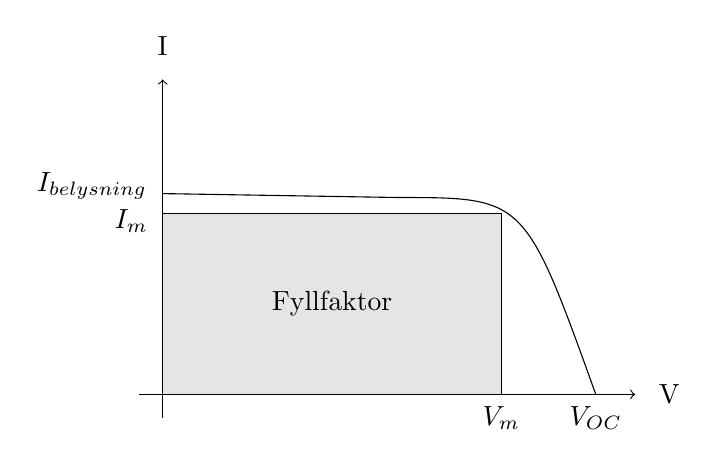
\begin{tikzpicture}

	\draw [->] (-0.3,0) -- (6,0) node [right=5pt]	{V};  % X-akse
	\draw [->] (0,-0.3) -- (0,4) node [above=5pt]	{I}; % Y-akse

	% Faktisk kurve
	\draw [-] (0,2.55) -- (3,2.5);
	\draw [-] (3,2.5) .. controls +(right:1.6cm) .. (5.5,0);
	
	% Fyllfaktor
	\node [draw, rectangle,fill=black!10,minimum height=2.3cm, minimum width=4.3cm] (FF) at (2.15,1.15) {Fyllfaktor};
	
	% Tekst
	\node at (-0.9,2.65) {$I_{belysning}$};
	\node at (-0.4,2.2) {$I_m$};
	\node at (4.3,-0.3) {$V_m$};
	\node at (5.5,-0.3) {$V_{OC}$};
	
	
\end{tikzpicture}

\caption{Str�m-spenningskarakterisitikken for en solcelle}%
\label{fig:fyllfaktor}%
\end{figure}

% Referanseliste
\clearpage
\bibliographystyle{plain}
\nocite{}
\bibliography{bibliography} % bibliography.bib

% Vedlegg
\clearpage
\appendix
\section{Transmisjonskurver}

\begin{figure}[H]%
\centering
%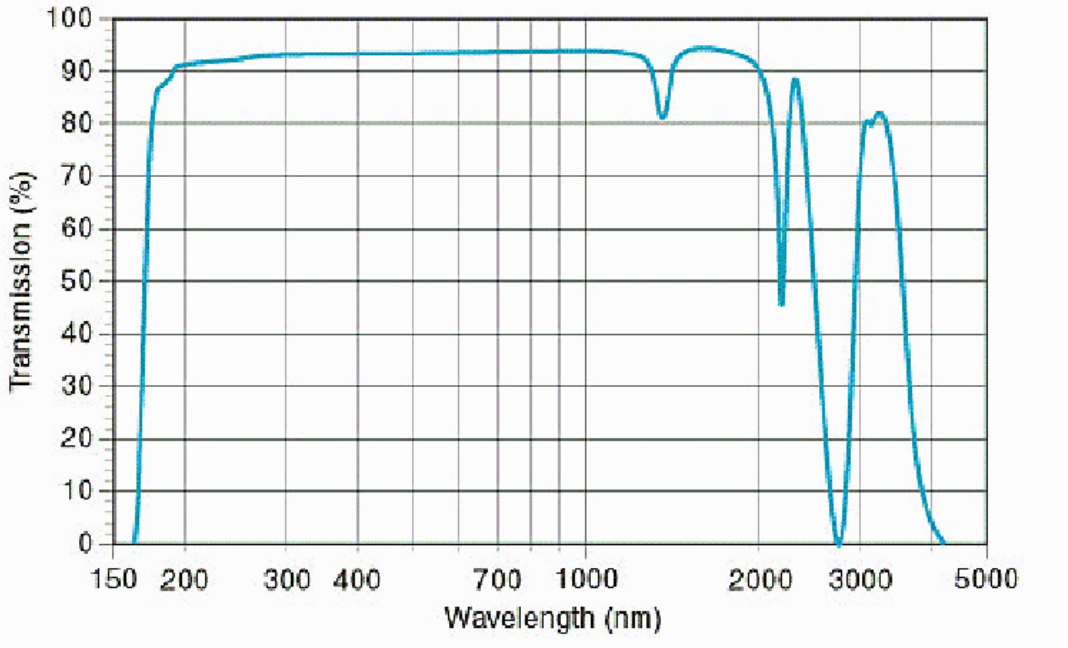
\includegraphics[width=10cm,bb=0 0 1068 648]{cryovindu}%
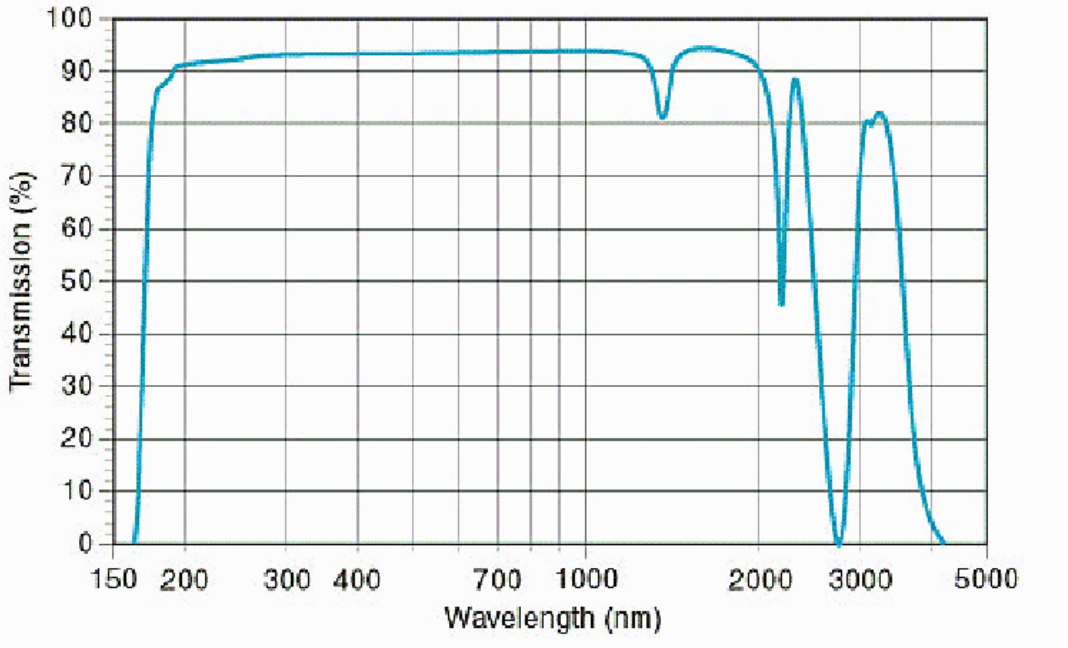
\includegraphics[width=10cm]{cryovindu}%
\caption{Transmisjon gjennom viduet til cryostaten \cite{cryostat} 27.10.2009}%
\label{fig:cryovindu}%
\end{figure}

\begin{figure}[H]%
\centering
%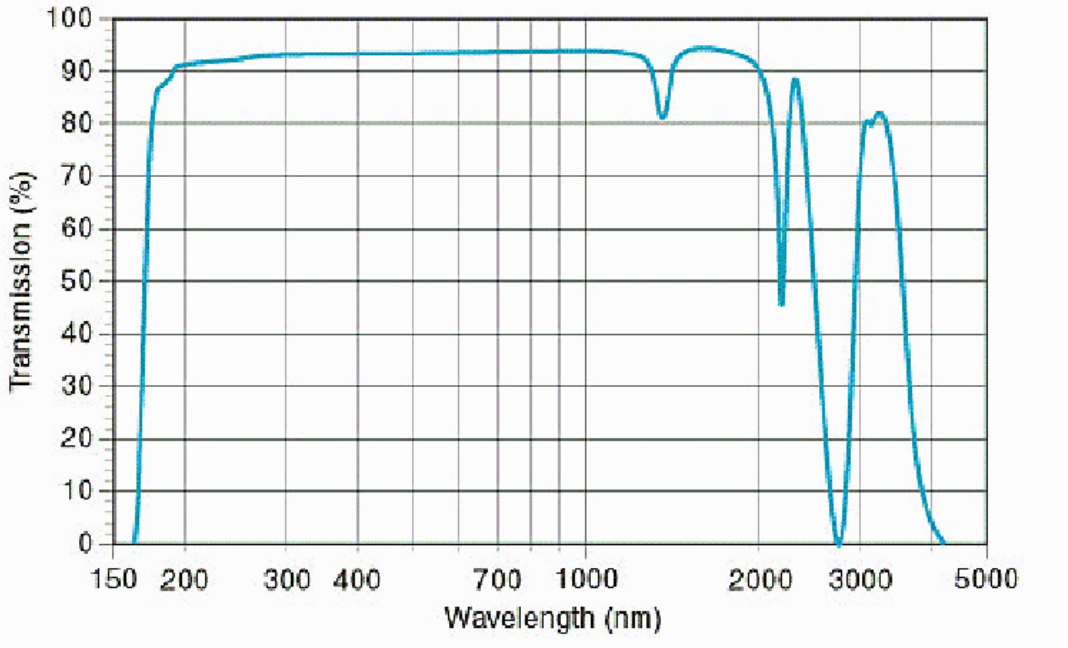
\includegraphics[width=10cm,bb=0 0 1068 648]{cryovindu}%
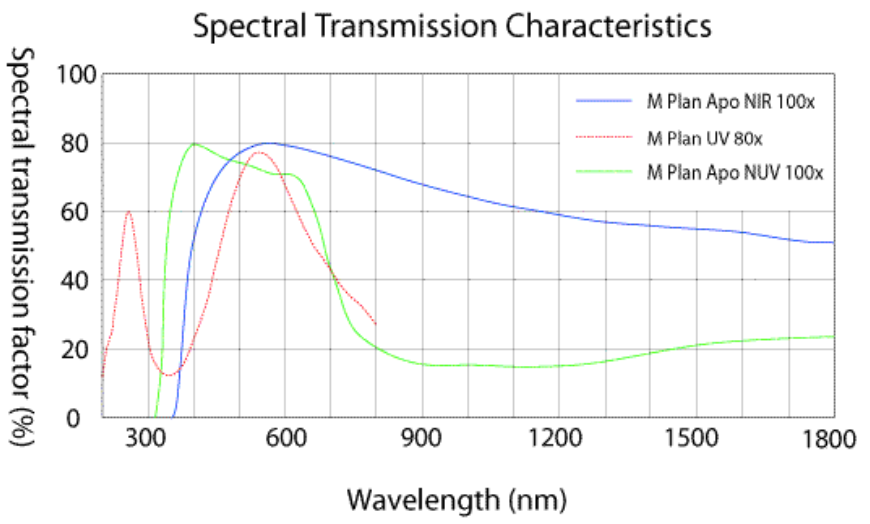
\includegraphics[width=10cm]{objektiv}%
\caption{Transmisjon gjennom objektivet \cite{objektiv} 08.12.2009}%
\label{fig:objektiv}%
\end{figure}

\begin{figure}[H]%
\centering
%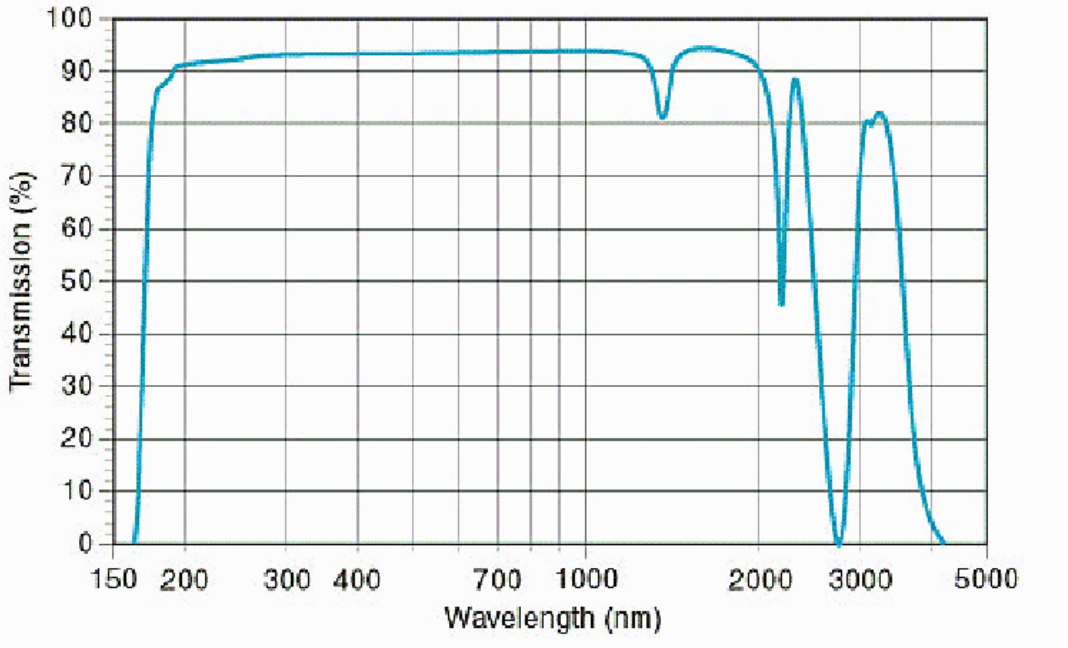
\includegraphics[width=10cm,bb=0 0 1068 648]{cryovindu}%
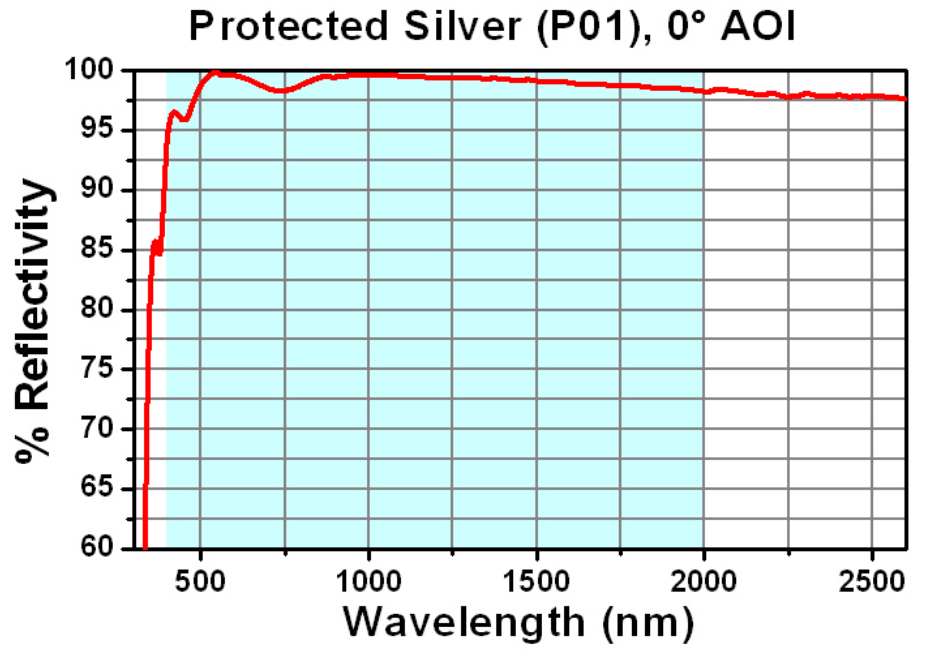
\includegraphics[width=10cm]{speil}%
\caption{Refleksjon for speil \cite{speil} 08.12.2009}%
\label{fig:speil}%
\end{figure}

\begin{figure}[H]%
\centering
%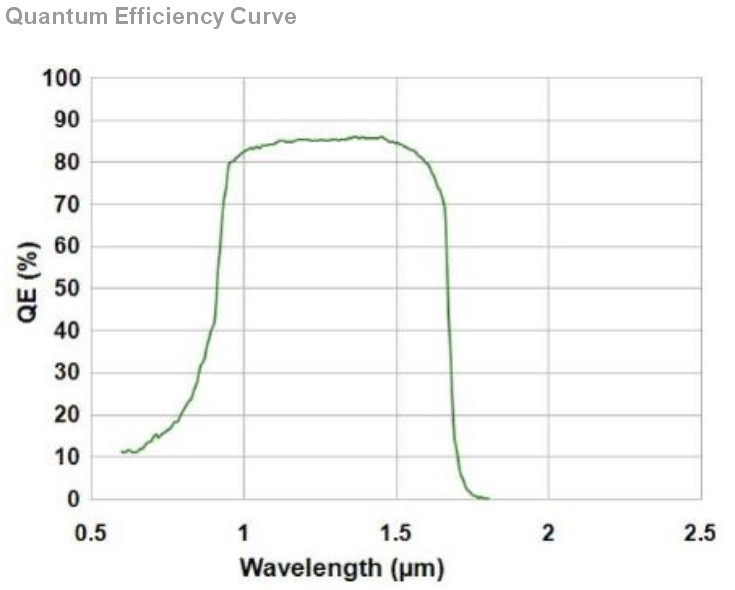
\includegraphics[width=10cm,bb=0 0 735 590]{kameragraf}%
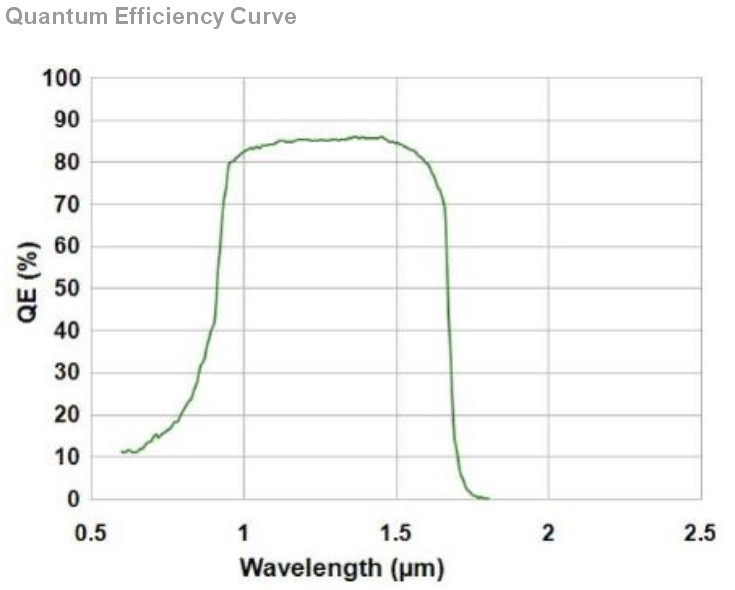
\includegraphics[width=10cm]{kameragraf}%
\caption{Kameraeffektivitet \cite{kamera} 27.10.2009}%
\label{fig:kameragraf}%
\end{figure}



\subsection{F�rste veibane}

\begin{figure}[H]%
\centering
%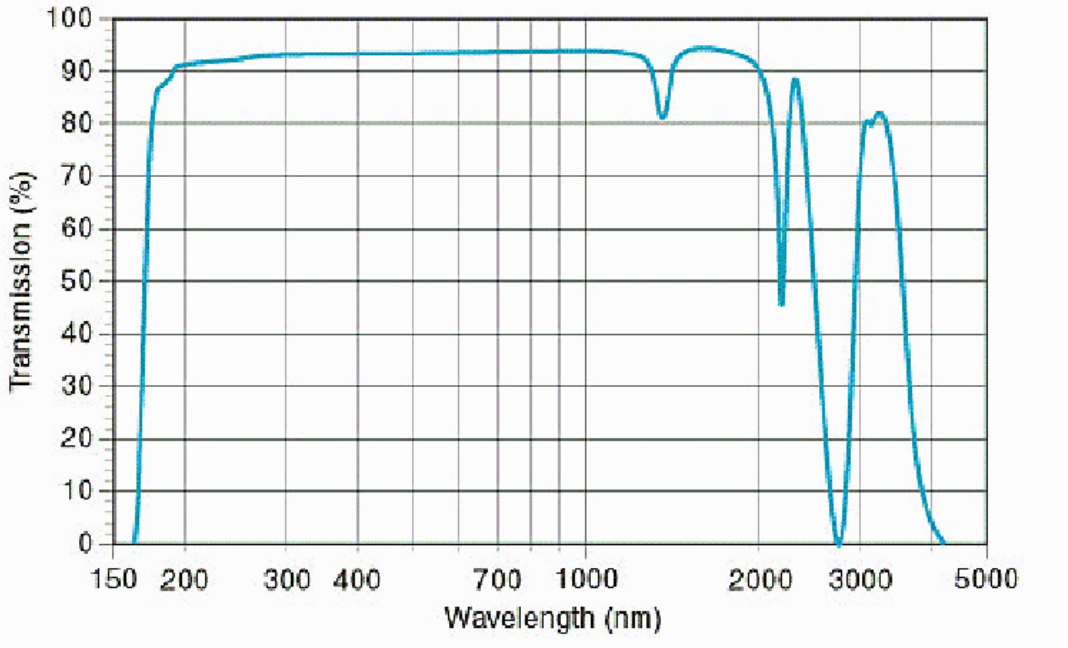
\includegraphics[width=10cm,bb=0 0 1068 648]{cryovindu}%
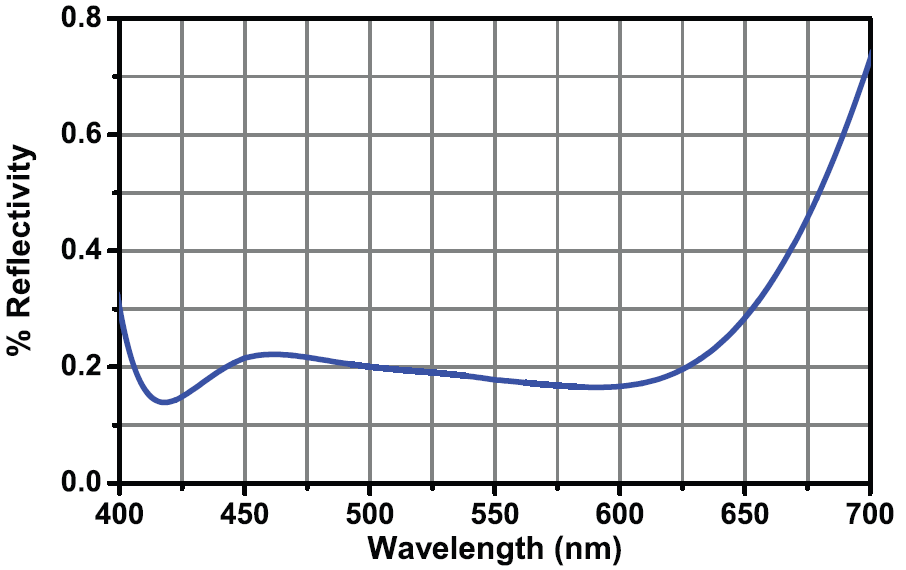
\includegraphics[width=10cm]{breamsplitter400-700nm}%
\caption[Beamsplitter 400-700nm]{Beamsplitter refleksjon fra datablad optimalisert for 400-700nm \cite{beamsplitter} 12.12.2009}%
\label{fig:beamsplitter400-700nm}%
\end{figure}

\begin{figure}[H]%
\centering
%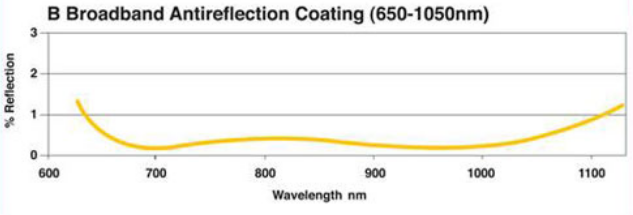
\includegraphics[width=10cm,bb=0 0 633 215]{old_linse}%
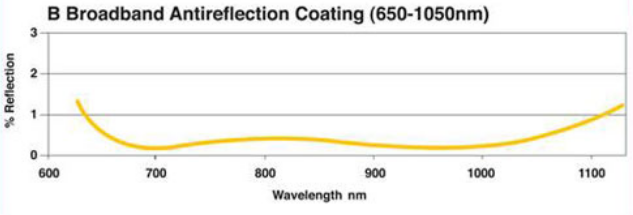
\includegraphics[width=\columnwidth]{old_linse}%
\caption{Transmisjon gjennom linse fra gammel veibane \cite{old_lens} 27.10.2009}%
\label{fig:linsetrans}%
\end{figure}

\subsection{Andre veibane}

\begin{figure}[H]%
\centering
%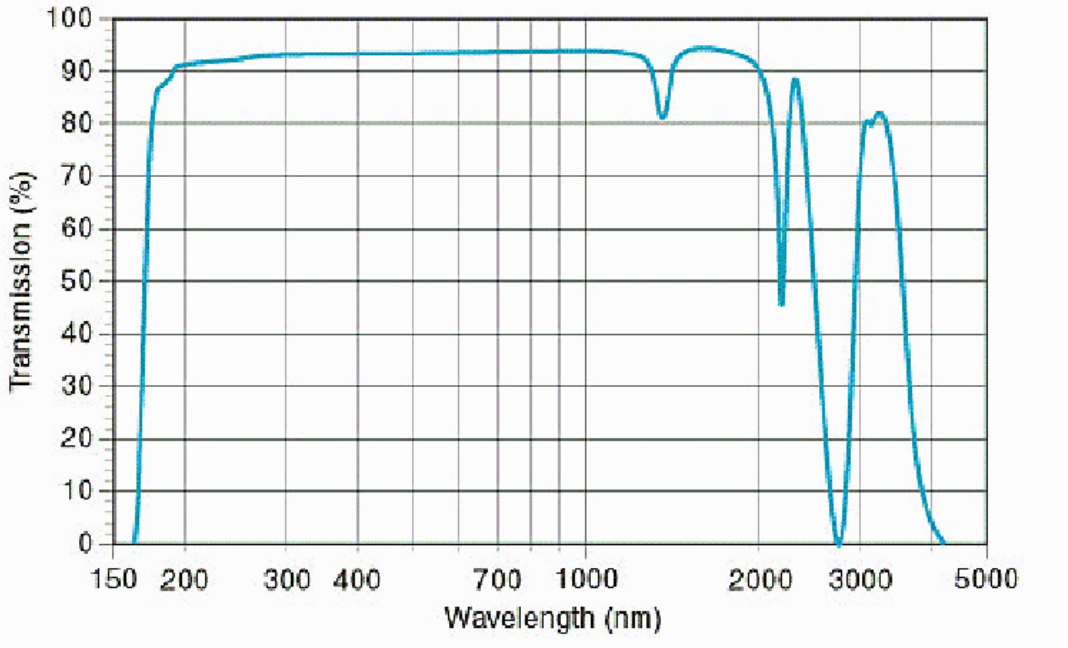
\includegraphics[width=10cm,bb=0 0 1068 648]{cryovindu}%
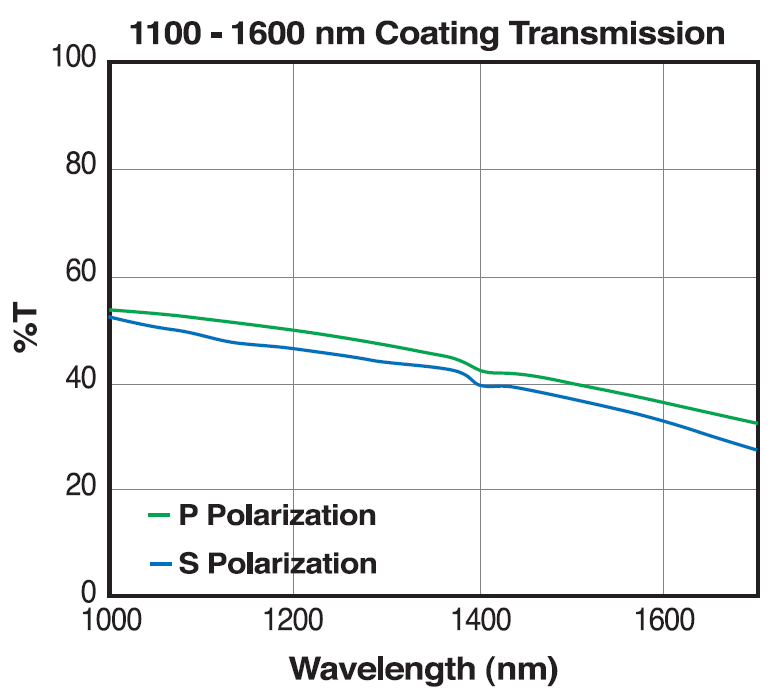
\includegraphics[width=10cm]{breamsplitter1100-1600nm}%
\caption[Beamsplitter 1100-1600nm]{Beamsplitter refleksjon fra datablad optimalisert for 1100-1600nm \cite{beamsplitter_ny} 12.12.2009}%
\label{fig:beamsplitter1100-1600nm}%
\end{figure}

\begin{figure}[H]%
\centering
%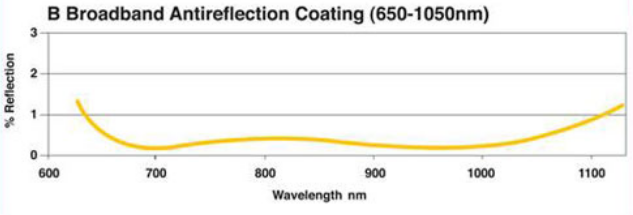
\includegraphics[width=10cm,bb=0 0 633 215]{old_linse}%
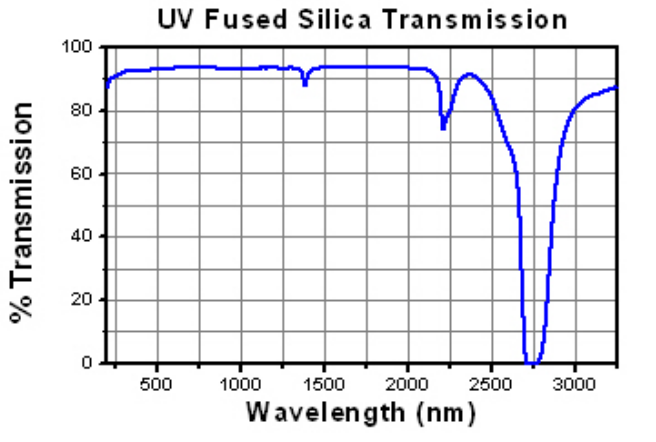
\includegraphics[width=10cm]{ny_linse}%
\caption{Transmisjon gjennom ny linse \cite{new_lens} 08.12.2009}%
\label{fig:linsetrans_ny}%
\end{figure}

\end{document}



